\chapter{Geometría Proyectiva}
\section{Contexto e idea}
Segun el programa de Erlegen, una geometría se basa en el estudio de invariantes
al aplicar unas ciertas transformaciones. Así tenemos que las geometrías están
"incluidas" en las superiores.

Así, la geometría euclidea, que estudia las transformaciones ortogonales, estaría
"incluída" en la geometría afín, que estudia las tansformaciones lineales. Aquí
se muestra una tabla con las distintas geometrías en la cual cada una esta
"incluída" en la anterior
\begin{center}
    \begin{tabular}{|c|c|}
        \hline Geometría & Transformaciones de estudio \\
        \hline \hline
        G. euclídea  & transformaciones ortogonales \\ \hline
        G. afín & transformaciones lineales \\ \hline
        G. proyectiva & proyectividades \\ \hline
        G. Algebraica & transformaciones por polinomios \\ \hline
        G. Analítica & transformaciones por funciones analíticas \\ \hline
        G. Diferencial & transformaciones por funciones de clase
        $\mathcal{C}^\infty$ \\ \hline
        Topología & transformaciones por funciones de clase $\mathcal{C}^0$\\ \hline
    \end{tabular}
\end{center}

\subsubsection{Problema matemático}
\begin{center}
    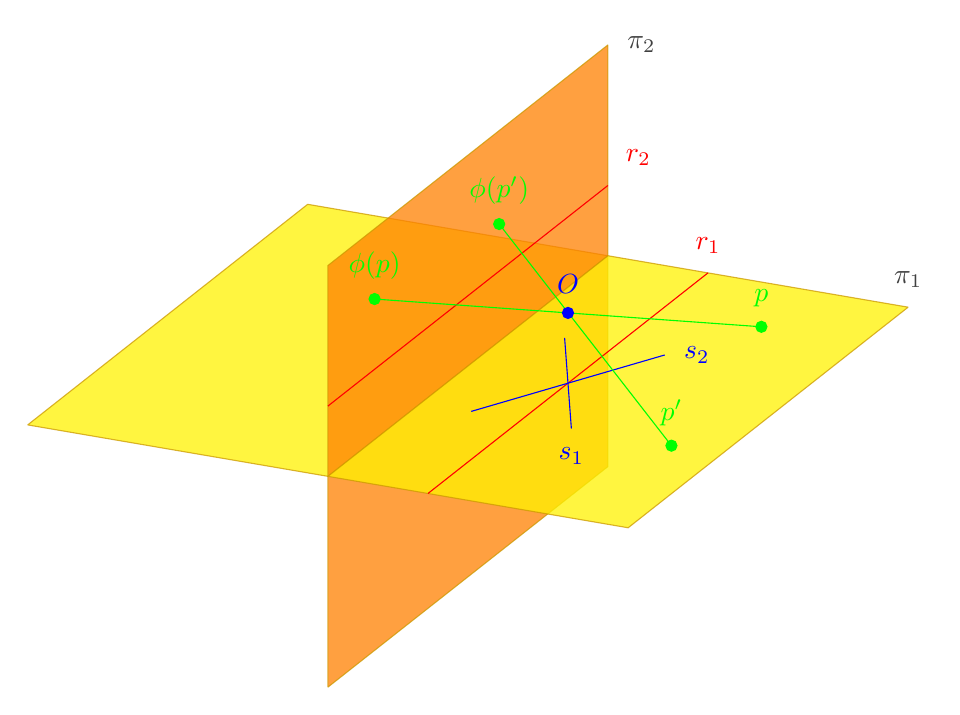
\begin{tikzpicture}
    \begin{axis}[%
    hide axis,
    width= 15 cm,
    enlargelimits=0.1
    ]

    \addplot3[patch, patch type=rectangle,opacity=.75,color=yellow]
    coordinates {(0,3,0) (-3,3,0) (-3,-3,0) (0,-3,0)};
    \addplot3[patch, patch type=rectangle,opacity=.75,color=orange]
    coordinates {(0,3,-3) (0,-3,-3) (0,-3,3) (0,3,3)}
    node[label={[black]right:$\pi_2$}]{};
    \addplot3[patch, patch type=rectangle,opacity=.75,color=yellow]
    coordinates {(3,-3,0) (0,-3,0) (0,3,0) (3,3,0)}
    node[label={[black]$\pi_1$}]{};

    \addplot3[color=blue,mark=*] coordinates {(1,0,1)}
    node[label=above:{$O$}]{};

    \draw [color=red] (axis cs:1,-3,0) -- (axis cs:1,3,0)
    node[label=$r_1$]{};
    \draw [color=red] (axis cs:0,-3,1) -- (axis cs:0,3,1)
    node[label=50:$r_2$]{};

    \draw [color=blue] (axis cs:0.5,1,0) -- (axis cs:1.5,-1,0)
    node[label=below:$s_1$]{};
    \draw [color=blue] (axis cs:0.5,-1,0) -- (axis cs:1.5,1,0)
    node[label=right:$s_2$]{};

    \addplot3[color=green,mark=*] coordinates {(2,2,0)}
    node[label=$p$]{};
    \addplot3[color=green,mark=*] coordinates {(0,-2,2)}
    node[label=$\phi(p)$]{};
    \draw [color=green] (axis cs:2,2,0) -- (axis cs:0,-2,2);

    \addplot3[color=green,mark=*] coordinates {(2.5,-1,0)}
    node[label=$p'$]{};
    \addplot3[color=green,mark=*] coordinates {(0,0.67,1.67)}
    node[label=$\phi(p')$]{};
    \draw [color=green] (axis cs:2.5,-1,0) -- (axis cs:0,0.67,1.67);
    \end{axis}
    \end{tikzpicture}
\end{center}
La idea básica del problema es enviar los puntos de $\pi_1$ a $\pi_2$ mediante la
siguiente aplicación
\[
\begin{aligned}
\phi \colon \pi_1 &\to \pi_2 \\
p &\mapsto \overline{p}_0 \cap \pi_2
\end{aligned}
\]
\begin{obs}
    \begin{enumerate}[i)]
        \item[]
        \item $\phi$ manda rectas a rectas
        \item\label{item:prob_r1} $\phi$ no esta definida en $r_1$
        \item\label{item:prob_r2} $r_2$ no esta en la imagen de $\phi$
        \item $\phi(s_1)$ y $\phi(s_2)$ son pararelas, por lo tanto, $\phi$ no
        mantiene el paralelismo
        \item $\phi$ no mantiene el tipo de cónica afín
    \end{enumerate}
\end{obs}
Veremos que la solucion para \ref{item:prob_r1} y \ref{item:prob_r2} consistirá
en añadir puntos en el $\infty$.

\section{Definición y caracterizaciones del espacio proyectivo}
\begin{defi}
    Sea $\k$ un cuerpo, $\E$ un $\k$-e.v. de $\dim n+1$. El espacio proyectivo asociado a $\E$ es
    \[\Po (\E) = \setb{\text{s.e.v. de } \dim 1 \text{ de } \E}\]
    Diremos que $\Po (\E)$ tiene dimensión $n$.
\end{defi}
\begin{obs}
    Se cumple $\Po (\E) = (\E \setminus \setb{0}) / \sim$, donde $v \sim v'  \iff \exists \lambda \neq 0, \ v' = \lambda v$ para
    $v, v' \in \E \setminus \setb{0}$.
\end{obs}
\begin{defi}
    Tenemos la siguiente aplicación $\pi$ dada por el paso al cociente.
    \[
    \begin{aligned}
    \pi \colon \E \setminus \setb{0} &\to \Po (\E)\\
    v &\mapsto \pi(v) = [v]\\
    \setb{\text{s.e.v. de } \dim 1 \text{ de } \E} &\leftrightarrow [v]
    \end{aligned}
    \]
\end{defi}
\begin{defi}
    A los elementos de $\Po (\E)$ los llamaremos puntos de $\Po (\E)$.
    \[p = \pi(v) = [v]\]
\end{defi}
\begin{obs}
    \begin{itemize}
        \item[]
        \item Si $\E$ no es relevante, $\Po^n = \Po (\E)$.
        \item Si queremos remarcar $\k$, $\Po_\k^n = \Po (\E)$.
        \item Normalmente $\Po+\k^n = \Po(\k^{n+1}) = (\k^{n+1} \setminus {0})/\sim$.
    \end{itemize}
\end{obs}
\begin{example}
    \begin{enumerate}
        \item []
        \item\label{item:po1r} $\Po^1_{\real}$.
        \begin{center}
        \begin{tikzpicture}
        \begin{axis}[%
        axis equal,
        enlargelimits=0,
        axis lines=center,
        ticks=none,
        ymin=-4,ymax=4,
        xmin=-4,xmax=4
        ]

        \addplot[color=orange] {2*x};
        \addplot[mark=*,color=red] coordinates {(1,2)};
        \addplot[color=orange] {0.5*x};
        \addplot[mark=*,color=red] coordinates {(1,0.5)};
        \addplot[color=orange] {4*x};
        \addplot[mark=*,color=red] coordinates {(1,4)};
        \addplot[color=orange] {-4*x};
        \addplot[mark=*,color=red] coordinates {(1,-4)};
        \addplot[color=orange] {-1*x};
        \addplot[mark=*,color=red] coordinates {(1,-1)};
        \addplot[color=orange] {-0.5*x};
        \addplot[mark=*,color=red] coordinates {(1,-0.5)};
        \addplot[color=orange] {12*x};

        \addplot[mark=*,color=white] coordinates {(0,0)};
        \addplot[mark=o] coordinates {(0,0)};

        \draw [color=red] (axis cs:1,-4) -- (axis cs: 1,1)
        node[label=right:$\bb{A}_\real^1$]{};
        \draw [color=red] (axis cs:1,1) -- (axis cs:1,4);
        \end{axis}
        \end{tikzpicture}
        \end{center}
        Cada objeto de $\Po^1_\real$ (rectas en naranja) tiene su equivalente en
        $\bb{A}^1_\real$ (puntos en rojo), a excepción de la recta $x=0$. Para solucionar
        este problema, podemos usar la siguiente representación
        \begin{center}
        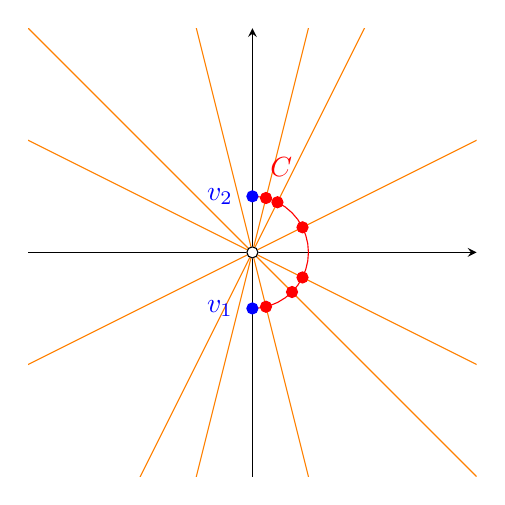
\begin{tikzpicture}
        \begin{axis}[axis equal image,
        axis lines=center,
        ticks=none,
        ymin=-4,ymax=4,
        xmin=-4,xmax=4]

            \addplot[color=orange] {2*x};
            \addplot[mark=*,color=red] coordinates {(0.447214,0.894428)};
            \addplot[color=orange] {0.5*x};
            \addplot[mark=*,color=red] coordinates {(0.894427,0.4472135)};
            \addplot[color=orange] {4*x};
            \addplot[mark=*,color=red] coordinates {(0.242536,0.970144)};
            \addplot[color=orange] {-4*x};
            \addplot[mark=*,color=red] coordinates {(0.242536,-0.970144)};
            \addplot[color=orange] {-1*x};
            \addplot[mark=*,color=red] coordinates {(0.707107,-0.707107)};
            \addplot[color=orange] {-0.5*x};
            \addplot[mark=*,color=red] coordinates {(0.894427,-0.4472135)};

            \addplot[mark=*,color=blue] coordinates {(0,-1)}
                node[label=left:$v_1$]{};
            \addplot[mark=*,color=blue] coordinates {(0,1)}
                node[label=left:$v_2$]{};

            \addplot[mark=*,color=white] coordinates {(0,0)};
            \addplot[mark=o] coordinates {(0,0)};


            \addplot [domain=-90:90, samples=21, color=red] ({cos(x)},{sin(x)})
                node[label=50:$C$]{};
        \end{axis}
        \end{tikzpicture}
        \end{center}
        Pero el problema ahora viene por que $v_1$ y $v_2$ corresponden al mismo elemento de
        $\Po^1_\real$. Lo podemos solucionar de la siguiente forma:
        \begin{center}
        \begin{tikzpicture}
        \begin{axis}[
            axis lines=center,
            axis equal,
            hide axis,
            enlargelimits=0.1
        ]
            \addplot [domain=-180:180, samples=50, color=red] ({cos(x)},{sin(x)});

            \addplot [mark=*,color=blue] coordinates {(-1,0)}
                node[label=left:$\infty$]{};
        \end{axis}
        \end{tikzpicture}
        \end{center}
        De tal forma que
        \[
            \bb{A}^1_\real \cup \setb{\infty} = \Po^1_\real = C/(v_1 \sim v_2)
        \]
        \item $\Po^2_{\real}$.
        \begin{center}
        \begin{tikzpicture}
        \begin{axis}[%
        axis equal,
        ticks=none,
        width= 10 cm,
        enlargelimits=0,
        axis lines=center,
        view={10}{20},
        ymin=-4,ymax=4,
        xmin=-4,xmax=4
        ]

            \draw [color=orange] (axis cs:-4,-4,-4) -- (axis cs:4,4,4);
            \addplot3 [mark=*,color=red] coordinates {(1,1,1)};
            \draw [color=orange] (axis cs:4,-2,-4) -- (axis cs:-4,2,4);
            \addplot3 [mark=*,color=red] coordinates {(1,-0.5,-1)};
            \draw [color=orange] (axis cs:-4,-2,0) -- (axis cs:4,2,0);
            \addplot3 [mark=*,color=red] coordinates {(1,0.5,0)};
            \draw [color=orange] (axis cs:-4,8,-12) -- (axis cs:4,-8,12);
            \addplot3 [mark=*,color=red] coordinates {(1,-2,3)};

            \addplot3[mark=*,color=white] coordinates {(0,0,0)};
            \addplot3[mark=o] coordinates {(0,0,0)};

            \addplot3 [patch, patch type=rectangle,opacity=.5,color=red]
            coordinates { (1,4,4) (1,-4,4) (1,-4,-4) (1,4,-4) }
            node[pin={[black]right:$\bb{A}^2_\real$}]{};
        \end{axis}
        \end{tikzpicture}
        \end{center}
        Cada objeto de $\Po^2_\real$ (rectas en naranja) tiene su equivalente en
        $\bb{A}^2_\real$ (puntos en rojo), a excepción de las rectas del plano $x=0$.
        Para solucionar este problema, procedemos de manera análoga a \ref{item:po1r}
        \begin{center}
        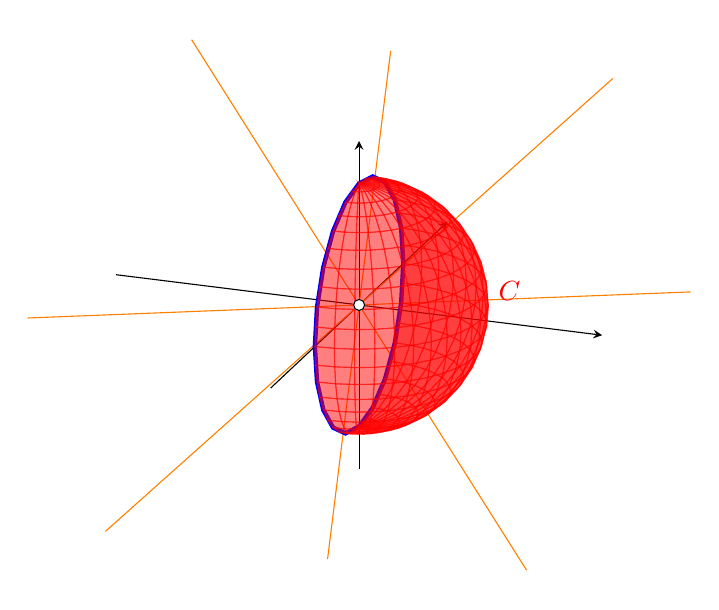
\begin{tikzpicture}
        \begin{axis}[%
        axis equal,
        ticks=none,
        width= 10 cm,
        enlargelimits=0,
        axis lines=center,
        view={20}{20},
        ymin=-2,ymax=2,
        xmin=-2,xmax=2
        ]
            \draw [color=orange] (axis cs:-4,-4,-4) -- (axis cs:4,4,4);
            \draw [color=orange] (axis cs:4,-2,-4) -- (axis cs:-4,2,4);
            \draw [color=orange] (axis cs:-4,-2,0) -- (axis cs:4,2,0);
            \draw [color=orange] (axis cs:-4,8,-12) -- (axis cs:4,-8,12);

            \addplot3[mark=*,color=white] coordinates {(0,0,0)};
            \addplot3[mark=o] coordinates {(0,0,0)};

            \addplot3[
            color=blue,
            samples=21,
            variable = \v,
            domain = 0:360,
            ultra thick
            ]
            ({0},{cos(v)},{sin(v)});

            \addplot3[%
            opacity = 0.5,
            surf,
            color=red,
            faceted color=red,
            z buffer = sort,
            samples = 21,
            variable = \u,
            variable y = \v,
            domain = -90:90,
            y domain = 0:180,
            ]
            ({cos(u)*sin(v)}, {sin(u)*sin(v)}, {cos(v)});

            \addplot3 [mark=none,color=red] coordinates {(1,0,0)}
                node[label=50:$C$]{};
        \end{axis}
        \end{tikzpicture}
        \end{center}
        De nuevo, nos encontramos con el problema de que hay elementos de $C$ (en azul)
        que se corresponden con el mismo elemento de $\Po^2_\real$, No obstante, podemos
        visualizarlo como
        \begin{center}
        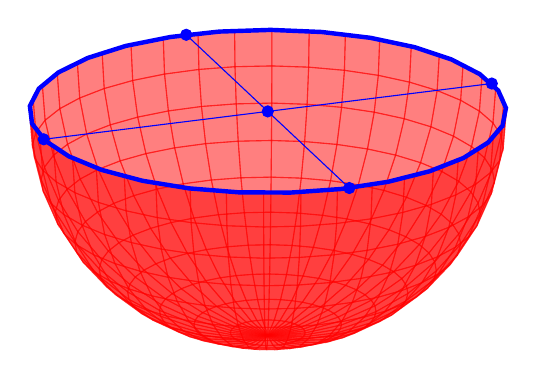
\begin{tikzpicture}
        \begin{axis}[axis equal,
        ticks=none,
        width= 10 cm,
        enlargelimits=0,
        axis lines=center,
        hide axis,
        view={10}{20},
        ymin=-1.2,ymax=1.2,
        xmin=-1.2,xmax=1.2
        ]
            \addplot3[%
            opacity = 0.5,
            surf,
            color=red,
            faceted color=red,
            z buffer = sort,
            samples = 21,
            variable = \u,
            variable y = \v,
            domain = 0:180,
            y domain = 90:270,
            ]
            ({cos(u)*sin(v)}, {sin(u)*sin(v)}, {cos(v)});

            \addplot3[
            color=blue,
            samples=30,
            variable = \v,
            domain = 0:360,
            ultra thick
            ]
            ({cos(v)},{sin(v)},{0});

            \addplot3 [mark=*,color=blue] coordinates {(0,0,0)};
            \addplot3 [mark=*,color=blue] coordinates {({cos(30)},{sin(30)},0)};
            \addplot3 [mark=*,color=blue] coordinates {({cos(210)},{sin(210)},0)};
            \draw (axis cs: {cos(30)}, {sin(30)}, 0) [color=blue] --
                (axis cs: {cos(210)}, {sin(210)}, 0);

            \addplot3 [mark=*,color=blue] coordinates {({cos(120)},{sin(120)},0)};
            \addplot3 [mark=*,color=blue] coordinates {({cos(300)},{sin(300)},0)};
            \draw (axis cs: {cos(120)}, {sin(120)}, 0) [color=blue] --
                (axis cs: {cos(300)}, {sin(300)}, 0);


        \end{axis}
        \end{tikzpicture}
        \end{center}
        Y unir los puntos azules antipolares. Aunque, si lo tratamos de imaginar, este
        objeto no cabe en $\real^3$.
        \item $\Po^1_{\cx} = (\cx^2 \setminus {0})/\sim \ = \cx \cup \setb{\infty} = S^2$. Las igualdades por el momento son
        por analogía o intuición, más adelante se demostrarán. Aunque nos podemos hacer una idea basándonos en la proyección
        estereográfica
        \begin{center}
        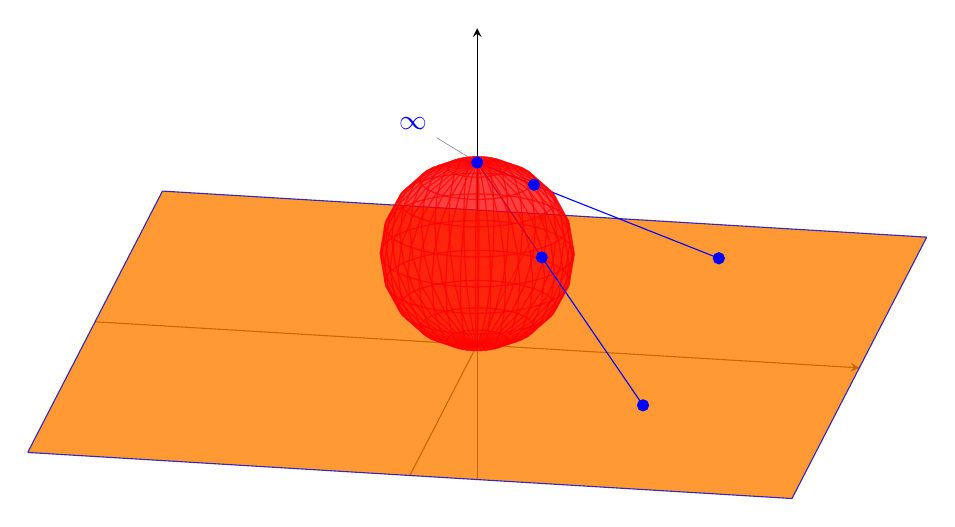
\begin{tikzpicture}
        \begin{axis}[axis equal,
        ticks=none,
        width=13 cm,
        enlargelimits=0,
        axis lines=center,
        view={10}{20},
        ymin=-4,ymax=4,
        xmin=-4,xmax=4]

            \addplot3[patch,color=orange, patch type=rectangle, opacity=0.8] coordinates
            {(4,4,0) (4,-4,0) (-4,-4,0) (-4,4,0)};

            \addplot3[color=blue,mark=*] coordinates {(0,0,2)} node[pin=150:{$\infty$}]{};

            \addplot3[mark=*,color=blue] coordinates {(2,3,0)};
            \addplot3[mark=*,color=blue] coordinates {(0.47,0.71,1.53)};
            \draw (axis cs:0,0,2) [color=blue] -- (axis cs:2,3,0);

            \addplot3[mark=*,color=blue] coordinates {(2,-1.5,0)};
            \addplot3[mark=*,color=blue] coordinates {(0.78,-0.59,1.22)};
            \draw (axis cs:0,0,2) [color=blue] -- (axis cs:0.78,-0.59,1.22);

            \addplot3[%
            opacity = 0.5,
            surf,
            color=red,
            faceted color=red,
            z buffer = sort,
            samples = 21,
            variable = \u,
            variable y = \v,
            domain = 0:180,
            y domain = 0:360,
            ]
            ({cos(u)*sin(v)}, {sin(u)*sin(v)}, {cos(v)+1});

            \draw (axis cs:0.78,-0.59,1.22)[color=blue] -- (axis cs:2,-1.5,0);

        \end{axis}
        \end{tikzpicture}
        \end{center}

        \item $\Po^2_{\z / 2}$ contiene $7$ puntos pues las rectas de $\z^3$ solo contienen el $0$ y un punto.
    \end{enumerate}
\end{example}
\begin{obs}
    Hemos enunciado la definición algebraica de $\Po_{\real}^{n}$. Existe una definición axiomática que no
    es igual en algunos casos patológicos.
\end{obs}

\section{Variedades lineales proyectivas}

\begin{defi}
    Sea $\E$ un $\k$-e.v. de dimensión $n+1$, sea $\Po^n = \Po(\E)$.
    Llamaremos variedad lineal (proyectiva) de dimensión $r$ a cualquier conjunto
    de la forma:
    \[V = \pi(H \setminus \setb{0})\]
    donde $H \subseteq \E$ es un subespacio vectorial de dimensión $r+1$.

    Por convención defnimos la siguiente notación:
    \[V = \pi(H \setminus \setb{0}) = \pi(H)\]
\end{defi}
\begin{example}
    \begin{itemize}
        \item []
        \item $\Po^n = \pi(\E)$ es una variedad lineal de dimensión $n$.
        \item $p \in \Po^n$, $p = \pi(v) = \pi([v])$ es una varidead lineal de dimensión $0$.
        \item $\emptyset = \pi({\emptyset_{\E}})$ es una variedad lineal de dimensión $-1$.
    \end{itemize}
\end{example}
\begin{defi}
    \begin{itemize}
        \item []
        \item $\dim V = 1 \longrightarrow$ Recta
        \item $\dim V = 2 \longrightarrow$ Plano
        \item $\dim V = n-1 \longrightarrow$ Hiperplano
    \end{itemize}
\end{defi}
\begin{lema}
    $V = \pi(H\setminus\setb{0}) \iff H \setminus \setb{0} = \pi^{-1}(V)$
\end{lema}
\begin{ej}
    Demostrar el lema anterior.
\end{ej}
\begin{obs}
    Hay una biyección
    \[\setb{\text{s.e.v. de } \E}
    \mathrel{\mathop{\rightleftarrows}^{\mathrm{\pi}}_{\mathrm{\pi^{-1}}}}
    \setb{\text{variedades lineales de } \Po(\E)}\]
    \begin{itemize}
        \item con dimension $r+1 \leftrightarrow r$
        \item $H_1 \subseteq H_2 \iff V_1 \subseteq V_2$ con $V_i=\pi(H_i)$
        \item Las operaciones $+$ y $\cap$ definidas para subespacios, se definen
        a traves de esta biyección a variedades.
    \end{itemize}
\end{obs}
\begin{prop}
    Sean $V_1, V_2 \subseteq \Po^n$ variedades lineales $\implies V_1 \cap V_2$ variedad lineal que verifica:
    \begin{itemize}
        \item $V_1 \cap V_2 \subseteq V_1, V_2$
        \item Si $W$ variedad lineal, $W \subseteq V_1, V_2 \implies W \subseteq V_1 \cap V_2$
    \end{itemize}
\end{prop}
\begin{proof}
    Veamos que: $V_1 \cap V_2 = \pi(H_1 \cap H_2)$ si $V_i = \pi(H_i)$ \\
    $\supseteq$
    \begin{gather*}
    \text{Si } v \in H_1 \cap H_2, p = [v] \in \pi(H_1), \pi(H_2) \implies p \in V_1 \cap V_2
    \end{gather*}
    $\subseteq$
    \begin{gather*}
        \text{Sea } p \in V_1 \cap V_2,
        \begin{rcases} p = [v_1], v_1 \in H_1 \\ p = [v_2], v_2 \in H_2 \end{rcases} \implies [v_1] = [v_2] \implies
        \exists \lambda \neq 0 \text{ t.q. } v_2 = \lambda v_1 \implies \\ \implies v_2 \in H_1 \implies v_2 \in H_1
        \cap H_2 \implies p = [v_2] \in \pi (H_1 \cap H_2)
    \end{gather*}
    El resto sigue de lo que sabemos de s.e.v.s.
\end{proof}
\begin{defi}
    Sean $V_1, V_2 \subseteq \Po^n$ variedades lineales, $V_i = \pi (H_i)$, definimos \textit{join} o variedad lineal generada como:
    \[
    V_1 \vee V_2 = \pi (H_1 + H_2)
    \]
\end{defi}
\begin{prop}
    \begin{itemize}
    \item[]
    \item $V_1, V_2 \subseteq V_1 \vee V_2$
    \item Sea $W$ una variedad lineal, $V_1, V_2 \subseteq W \implies V_1 \vee V_2 \subseteq W$
    \end{itemize}
\end{prop}
\begin{proof}
    Propiedades de la suma de s.e.v.
\end{proof}
\begin{prop}
    Sean $V_1, V_2 \subseteq \Po^n$ variedades lineales:
    \begin{itemize}
        \item $V_1 \subseteq V_2 \implies \dim \left( V_1\right) \leq \dim \left( V_2 \right)$
        \item Si $V_1 \subseteq V_2$ y $\dim \left( V_1 \right) = \dim \left( V_2 \right) \implies V_1 = V_2$
    \end{itemize}
\end{prop}
\begin{prop}[Fórmula de Grassmann]
    \[ \dim \left( V_1 \cap V_2 \right) + \dim \left( V_1 \vee V_2 \right) = \dim \left( V_1 \right) + \dim \left( V_2 \right) \]
\end{prop}
\begin{proof}
    Propiedades s.e.v.
\end{proof}
\begin{example}
    \begin{enumerate}
        \item[]
        \item $\Po^2 \quad V_1, V_2$ rectas, tenemos que $\dim \left( V_1 \cap V_2 \right) + \dim \left( V_1 \vee V_2 \right) = 2$ (Grassmann).
        \begin{center} \begin{tabular}{|c|c|c|}
            \hline $\dim \left( V_1 \cap V_2 \right)$ & $1 \leq \dim \left( V_1 \vee V_2 \right) \leq 2$  & Posición relativa \\
            \hline \hline
            0 & 2 & Se cortan en un punto \\ \hline
            1 & 1 & Son la misma recta\\ \hline
        \end{tabular} \end{center}
        Por tanto, dos rectas en un plano, o se cruzan o son la misma.
        \item $\Po^3 \quad V_1, V_2$ rectas, tenemos que $\dim \left( V_1 \cap V_2 \right) + \dim \left( V_1 \vee V_2 \right) = 2$ (Grassmann).
        \begin{center} \begin{tabular}{|c|c|c|}
            \hline $\dim \left( V_1 \cap V_2 \right)$ & $1 \leq \dim \left( V_1 \vee V_2 \right) \leq 3$  & Posición relativa \\
            \hline \hline
            -1 & 3 & Se cruzan \\ \hline
            0 & 2 & Se cortan en un punto $\left( V_1 \vee V_2 \cong \Po^2 \right)$ \\ \hline
            1 & 1 & Son la misma recta\\ \hline
        \end{tabular} \end{center}
        \item $\Po^3 \quad V_1, V_2$ planos, tenemos que $\dim \left( V_1 \cap V_2 \right) + \dim \left( V_1 \vee V_2 \right) = 4$ (Grassmann).
        \begin{center} \begin{tabular}{|c|c|c|}
            \hline $\dim \left( V_1 \cap V_2 \right)$ & $2 \leq \dim \left( V_1 \vee V_2 \right) \leq 3$  & Posición relativa \\
            \hline \hline
            1 & 3 & Se cortan en una recta \\ \hline
            2 & 2 & Son el mismo plano\\ \hline
        \end{tabular} \end{center}
        \item $\Po^3 \quad V_1$ plano, $V_2$ recta, tenemos que $\dim \left( V_1 \cap V_2 \right) + \dim \left( V_1 \vee V_2 \right) = 3$ (Grassmann).
        \begin{center} \begin{tabular}{|c|c|c|}
            \hline $\dim \left( V_1 \cap V_2 \right)$ & $2 \leq \dim \left( V_1 \vee V_2 \right) \leq 3$  & Posición relativa \\
            \hline \hline
            0 & 3 & Se cortan en un punto \\ \hline
            1 & 2 & $V_2 \subseteq V_1$ \\ \hline
        \end{tabular} \end{center}
    \end{enumerate}
\end{example}
\begin{prop}
    Sean $p \in \Po^n, r, V, H \subseteq \Po^n$ (recta, variedad lineal, hiperplano, respectivamente).
    \begin{enumerate}
        \item $\dim \left( V \vee p \right) = \text{ ó } \begin{cases} \dim V & (\iff p \in V) \\ \dim V + 1 & (\iff p \notin V) \end{cases}$
        \item $\dim \left( r \cap H \right) = \text{ ó } \begin{cases} 1 & (\iff r \subseteq H) \\ 0 & (\iff r \nsubseteq H) \end{cases}$
    \end{enumerate}
\end{prop}
\begin{proof}
    Fórmula de Grassmann.
\end{proof}
\begin{defi}
    Sean $V_1, V_2 \subseteq \Po^n, (V_i = \pi \left( H_i \right)$ variedades lineales, $V_1$ y $V_2$ son suplementarias $\iff H_1$ y $H_2$
    son complementarios.
\end{defi}
\begin{obs}
    \begin{gather*}
        V_1, V_2\text{ suplementarias }\iff H_1 \oplus H_2 = \E \iff \left. \begin{cases} (1) & H_1 + H_2 = \E \\ (2) & H_1 \cap H_2 = \emptyset \end{cases} \right\} \iff \\
        \iff \begin{cases} (1) & V_1 \vee V_2 = \Po^n \\ (2) & V_1 \cap V_2 = \emptyset \end{cases} \\
    \end{gather*}
\end{obs}
\begin{prop}
    Sean $V_1, V_2 \subseteq \Po^n$ variedades lineales:
    \begin{enumerate}
        \item $V_1, V_2$ son suplementarias $\implies \dim V_1 + \dim V_2 = n-1$
        \item Si $\dim V_1 + \dim V_2 = n-1$
        \[
        V_1, V_2 \text{ suplementarias} \iff V_1 \vee V_2 = \Po^n \iff V_1 \cap V_2 = \emptyset
        \]
    \end{enumerate}
\end{prop}
\begin{proof}
    \begin{enumerate}
        \item[]
        \item $V_1, V_2$ suplementarias $\iff H_1, H_2$ complementarios $\implies \overbrace{\dim H_1}^{\dim V_1 + 1} +
        \overbrace{\dim H_2}^{\dim V_2 + 1} = \dim \E = n+1$
        \item Fórmula de Grassmann.
    \end{enumerate}
\end{proof}
\begin{defi}
    Sea $\Po^n = \real(\E )$, y sean $p_0, \dots, p_m \in \Po^n$ tal que $p_i = [v_i], v_i \in \E$, decimos que $p_0, \dots,
    p_m$ son linealmente independientes (l.i.) $\iff v_0, \dots, v_m \in \E$ son linealmente independientes.
\end{defi}
\begin{obs}
    La independencia lineal no depende de los representantes elegidos.
\end{obs}
\begin{example}
    $\Po^2_\real = \Po(\real^3)$. Sean $p_0 = [(1,1,0)], p_1 = [(0,1,1)], p_2 = [(2,3,1)]$. Entonces $p_0$ y $p_1$ son linealmente
    independientes, pero $p_0, p_1, p_2$ son linealmente dependientes.
\end{example}
\begin{prop}
    Sean $p_0, \dots, p_m \in \Po^n$ puntos y $V \subseteq \Po^n$ una variedad lineal:
    \begin{enumerate}
        \item $\dim\left( p_0 \vee \dots \vee p_m \right) \leq m$.
        \item $\dim\left( p_0 \vee \dots \vee p_m \right) = m \iff p_0, \dots, p_m$ son linealmente independientes.
        \item $\dim V = m \iff \exists p_0, \dots, p_m \in V$ linealmente independientes tales que $V = p_0 \vee \dots \vee p_m
            \iff \forall p_0, \dots, p_m \in V \text{ linealmente independientes}, V = p_0 \vee \dots \vee p_m$.
    \end{enumerate}
\end{prop}
\begin{proof}
    Inmediata a partir de propiedades de s.e.v..
\end{proof}
\begin{defi}
    $p_0, \dots, p_r \in \Po^n (r \geq n)$ están en posición general $\iff n+1$ puntos cualesquiera de ellos son l.i..
\end{defi}

\section{Sistemas de referencia proyectivos. Coordenadas proyectivas}

\begin{obs}
    $\Po^n = \Po(\E)$. Sea $B = \{v_0, \dots, v_n\}$ base de $\E$:
    \begin{center} \begin{tabular}{ccc}
        $p = [v] = [\lambda v] \qquad $ &
        $(v)_B = \begin{pmatrix} x_0 \\ \vdots \\ x_n \end{pmatrix}\qquad $&
        $(\lambda v)_B = \begin{pmatrix} \lambda x_0 \\ \vdots \\ \lambda x_n \end{pmatrix} \qquad$
    \end{tabular} \end{center}
    Vemos que las coordenadas estarían definidas salvor por multiplicar por $\lambda$.
\end{obs}
\begin{defi}
    $\Po^n = \Po(\E)$
    \begin{enumerate}
        \item Un sistema de referencia proyectivo en $\Po^n$ es:
            \[ R= \{ p_0, \dots, p_n; \overline{p} \} \]
            Donde $p_0, \dots, p_n, \overline{p}$ están en posición general.
            \begin{itemize}
                \item $\{ p_0, \dots, p_n \}$ son los vertices de $R$
                \item $\overline{p}$ es el punto unidad
            \end{itemize}
        \item Fijado un sistema de referencia $R$. Sea $B = \{ u_0, \dots, u_n \}$ base de $\E$. Diremos que $B$ está adaptada a $R$ si y solo si:
            \[ \begin{cases} p_i = [u_i], \forall i = 0, \dots, n \\ \overline{p} = [u_0 + \dots + u_n ] \end{cases} \]
        \item \textit{Asignación de coordenadas proyectivas} \\
            $\Po^n = \Po(\E)$, Sea $R = \{ p_0, \dots, p_n; \overline{p} \}$, y $B = \{u_0, \dots, u_n\}$ una base adaptada. Sea $q \in \Po^n, q = [v]$, entonces
            $q_R = v_B$. (Hace falta ver que la definición es consistente)
    \end{enumerate}
\end{defi}
\begin{prop}
    Sea $R$ un sistema de referencia en $\Po^n$. Sean $B_1 = \{ u_0, \dots, u_n\}, B_2 = \{ u'_0, \dots u'_n \}$ bases adaptadas a $R$. Sea $q = [v] \in \Po^n$,
    entonces $\exists \lambda \neq 0$ tal que $v_{B_2} = \lambda v_{B_1}$.
\end{prop}
\begin{proof}
    $p_i = [u_i] = [u'_i], \forall i = 0, \dots, n$. Por tanto, $\exists \lambda \neq 0$ tal que $u'_i= \lambda_i u_i, \forall i = 1, \dots, n$. Por otro lado,
    \begin{gather*}
        \overline{p} = [u_0 + \dots + u_n] = [u'_0 + \dots + u'_n] \implies \exists \lambda \neq 0 \text{ tal que } u'_0 + \dots + u'_n = \\ = \lambda_0 u_0 + \dots + \lambda_n u_n = \lambda (u_0 + \dots + u_n)
        \stackrel{B_1 \text{ base}}{\implies} \lambda_i = \lambda \text{ } \forall i = 1, \dots, n
    \end{gather*}
\end{proof}
\begin{obs}
    $R = \{ p_0, \dots, p_n; \overline{p} \}$ en $\Po^n$
    \begin{enumerate}
        \item $q \in \Po^n, q_R = (a_0, \dots, a_n) = \lambda (a_0, \dots, a_n) \stackrel{\text{notación}}{=} (a_0 : \dots : a_n)$ $\forall \lambda \neq 0$
        \item Ejemplos: \\ $\begin{aligned} (p_0&)_R = (1:0:\dots:0) \\ \vdots& \\ (p_n&)_R = (0:\dots:0:1) \end{aligned}$
        \item $q_R = (0: \dots : 0)$ no existe.
        \item Sea $\Po^2_\real = \Po(\real^3), R = \{ p_0, p_1, p_2; \overline{p} \} = \left\{ [(1,1,0)], [(1,0,1)], [(0,1,1)]; [(3,3,2)]\right\}$, entonces $B = \left\{ [(1,1,0)], [(1,0,1)], [(0,1,1)] \right\}$ no es una base
            adaptada, para que lo sea, debemos multiplicar $v_0, v_1, v_2$ por $\lambda_0, \lambda_1, \lambda_2$ tales que $\overline{p} = \lambda_0 p_0 + \lambda_1 p_1 + \lambda_2 p_2$. En este caso:
            \[
                \begin{cases} \lambda_0 + \lambda_1 = 3 \\ \lambda_0 + \lambda_2 = 3 \\ \lambda_1 + \lambda_2 = 2 \end{cases} \iff \begin{cases} \lambda_0 = 2 \\ \lambda_1 = 1 \\ \lambda_2 = 1 \end{cases}
            \]
            Y el sistema de referencia con la base $B$ adaptada es: \[ R' = \left\{ [(2,2,0)], [(1,0,1)], [(0,1,1)]; [(3,3,2)]\right\} \]
    \end{enumerate}
\end{obs}

%%%%%%%%%%%%%%%%%%%%%%%%%%%%%%%%%%
% YA NO FALTAN LUNES Y MIERCOLES %
%%%%%%%%%%%%%%%%%%%%%%%%%%%%%%%%%%
%%%%%%%%%%%%%%%%%%%%%%%%%%%%%%%%%%
%      ¿POR QUÉ LEES ESTO?       %
%%%%%%%%%%%%%%%%%%%%%%%%%%%%%%%%%%

\begin{example}
    Consideremos el espacio $\Po^2_{\real}$, un sistema de referencia $\R = \{ p_0, p_1, p_2; \overline{p}\}$, con
    $p_0 = [(1, 1, 0)]$, $p_1 = [(1, 0, 1)]$, $p_2 = [(0, 1, 1)]$ y $\overline{p} = [(3,3,2)]$.
    Queremos encontrar $B = \{u_0, u_1, u_2\}$ una base adaptada, es decir, que cumpla $\overline{p} = [u_0+u_1+u_2]$
    y que $p_i = [u_i]$. Comprobamos que para la base $B = \left \{ (2,2,0)^t, (1,0,1)^t, (0,1,1)^t \right \}$, se cumple
    \[(p_0)_{\R} = (1:0:0) \quad (p_1)_{\R} = (0:1:0)\]
    \[(p_2)_{\R} = (0:0:1) \quad (\overline{p})_{\R} = (1:1:1)\]
    El punto $q = [(3, 2, 1)]$ tiene las coordenadas $q_{\R} = w_B = (1:1:0)$, que, en un abuso de notación,
    escribiremos como $(1, 1, 0)$.
\end{example}

\begin{prop}
    Sean $\R_1, \R_2$ sistemas de referencia de $\Po^n$. Sea $q \in \Po^n$.
    \begin{enumerate}[i)]
        \item $\exists S \in \mathcal{M}_{n+1}(\k)$ invertible tal que $q_{\R_1} = S q_{\R_2}$
        (matriz del cambio de sistema de referencia).
        \item Sean $B_1, B_2$ bases adaptadas a $\R_1, \R_2$ respectivamente. Podemos coger $S=S_{B_2, B_1}$.
        \item Cualquier matriz de cambio de referencia es de la forma $S=\lambda S_{B_2, B_1} \ (\lambda \neq 0)$.
    \end{enumerate}
\end{prop}
\begin{proof}
    Cambio de base en $\E$.
\end{proof}
\begin{obs}
    Sea $\R$ sistema de referencia en $\Po^n$, y $B$ una base adaptada a éste. Las variedades lineales se pueden describir con
    \begin{itemize}
        \item Ecuaciones paramétricas: Sea $V \subseteq \Po^n$ una variedad lineal de $\dim m$. Entonces
        $\exists p_0, \dots, p_m \in V$ linealmentes independientes tales que $V = p_0 \vee \dots \vee p_m$ y para $q \in \Po^n$
        \[
            q \in V \iff w \in F \iff
            \begin{cases}
                \exists \alpha_0, \dots, \alpha_m \in \k \\
                w_B = \alpha_0(v_0)_B + \dots + \alpha_m(v_m)_B
            \end{cases}
            \iff
            \]
        \[
            \iff
            \begin{cases}
                \exists \alpha_0, \dots, \alpha_m \in \k \\
                q_R = \alpha_0 (p_0)_R + \dots + \alpha (p_m)_R
            \end{cases}
        \]
        Donde $V = \pi(F)$, $p_i = \pi(v_i)$, y $q = \pi(w)$.
        \item Ecuaciones implícitas: Las ecuaciones implícitas de $V$ en $\R$ coinciden con las ecuaciones implícitas de $F$ en
        $B$. Es decir, existe una matriz $A$ tal que los vectores $w_B = \begin{pmatrix} x_0 \\ \vdots \\ x_n \end{pmatrix}$ que cumplen $A \begin{pmatrix} x_0 \\ \vdots \\ x_n \end{pmatrix} =
        \begin{pmatrix} 0 \\ \vdots \\ 0 \end{pmatrix}$ son todos los pertenecientes a $F$ y los puntos
        $q_R = \begin{pmatrix} x_0 \\ \vdots \\ x_n \end{pmatrix}$ que cumplen $A \begin{pmatrix} x_0 \\ \vdots \\ x_n \end{pmatrix} =
        \begin{pmatrix} 0 \\ \vdots \\ 0 \end{pmatrix}$ son todos los pertenecientes a $V$.
    \end{itemize}
\end{obs}
\begin{obs}
        Sea $\E$ un $\k$-e.v. de dimensión $n+1$, $F$ un subespacio vectorial de dimensión $m+1$, $\Po^n = \Po(\E)$ y $V = \pi(F)$
        una variedad lineal.
        Entonces
        \[\dim V = \dim F - 1 = \dim E - \rg A - 1 = n+1 - \rg A - 1 \implies m = \dim V = n - \rg A\]
\end{obs}
\begin{obs}
    \begin{itemize}
        \item[]
        \item Para convertir de ecuaciones implícitas a paramétricas se debe resolver el sistema de ecuaciones homogéneo.
        \item Para convertir de ecuaciones paramétricas a implícitas se debe imponer
        \[
            \rg
            \left(
            \begin{array}{ccc|c}
                (p_0)_R & \dots & (p_m)_R & \begin{array}{c}x_0 \\ \vdots \\ x_n \end{array} \\
            \end{array}
            \right)
            =
            \rg
            \left(
            \begin{array}{ccc}
                (p_0)_R & \dots & (p_m)_R\\
            \end{array}
            \right)
        \]
    \end{itemize}
\end{obs}
\begin{example}
    Consideremos el espacio $\Po^2_{\real}$ con un sistema de referencia $\R = \{p_0, p_1, p_2, \overline{p}\}$, y los puntos
    $(q_0)_{\R} = (1, 1, 1)$ y $(q_1)_{\R} = (1, 2, 0)$. Encontremos las ecuaciones paramétricas e implícitas de la recta
    $V = q_0 \vee q_1$.
    \begin{itemize}
        \item Dado que los puntos son dados directamente y se hace su join, las ecuaciones paramétricas son tan solo
        las combinaciones lineales de $q_0$ y $q_1$. Más formalmente, si $(q)_{\R} = \begin{pmatrix} x_0 \\ x_1 \\ x_2 \end{pmatrix}$,
        se cumple
        \[
            q \in V \iff \exists \alpha_0, \alpha_1 \text{ t.q. } \begin{pmatrix} x_0 \\ x_1 \\ x_2 \end{pmatrix}
            = \alpha_0 \begin{pmatrix} 1 \\ 1 \\ 1 \end{pmatrix} + \alpha_1 \begin{pmatrix} 1 \\ 2 \\ 0 \end{pmatrix}
        \]
        \item Para encontrar las ecuaciones implícitas de esta variedad, imponemos que $(x_0, x_1, x_2)$ sea combinación
        lineal de $q_0$ y $q_1$, es decir,
        \[
            q \in V \iff
            \rg
            \left(
            \begin{array}{cc|c}
                1 & 1 & x_0 \\
                1 & 2 & x_1 \\
                1 & 0 & x_2 \\
            \end{array}
            \right)
            =
            \rg
            \left(
            \begin{array}{cc}
                1 & 1 \\
                1 & 2 \\
                1 & 0 \\
            \end{array}
            \right)
            =
            2
            \iff
            \begin{vmatrix}
                1 & 1 & x_0 \\
                1 & 2 & x_1 \\
                1 & 0 & x_2
            \end{vmatrix}
            =
            0
        \]
    \end{itemize}
    Consideremos ahora la recta $V'$ dada por $x_0+x_1+x_2 = 0$. Para encontrar su expresión paramétrica,
    debemos resolver este sistema de ecuaciones. En este caso, podemos encontrar dos soluciones linealmente
    independientes y expresar todas las soluciones como combinaciones lineales de estas.
    \[\begin{pmatrix} x_0 \\ x_1 \\ x_2 \end{pmatrix} = \beta_0 \begin{pmatrix} 1 \\ -1 \\ 0 \end{pmatrix}
    + \beta_1 \begin{pmatrix} 0 \\ 1 \\ -1 \end{pmatrix}\]
    En este mismo ejemplo, $p_0 \vee p_1 : x_2 = 0$, $p_2 \vee \overline{p} : x_1-x_0 = 0$ y
    $(p_0 \vee p_1) \cap (p_2 \vee \overline{p}) = (1, 1, 0)$. Análogamente para los demás índices.
\end{example}

\begin{example}
    Consideremos $\Po^2_{\sfrac{\z}{2}}$. Sus puntos se pueden expresar como $(a, b, c) \  a,b,c \in \sfrac{\z}{2}$.
    Podemos representarlo como

    \begin{center}
\begin{tikzpicture}[scale=1]
    \draw (0,0) coordinate (A) --
    (3,0) coordinate (B)--
    ($ (3*0.5,{3*sin(60)}) $) coordinate (C) -- cycle;
    \coordinate (O) at
    (barycentric cs:A=1,B=1,C=1);
    \draw (O) circle [radius=3*1.717/6];
    \draw (C) -- ($ (A)!.5!(B) $) coordinate (LC);
    \draw (A) -- ($ (B)!.5!(C) $) coordinate (LA);
    \draw (B) -- ($ (C)!.5!(A) $) coordinate (LB);
    \node[draw,
    circle,
    fill=cyan,
    inner sep=1.5pt, label={-90:\tiny $(0, 0, 1)$}] at (A) {};
    \node[draw,
    circle,
    fill=cyan,
    inner sep=1.5pt, label={-90:\tiny $(0, 1, 0)$}] at (B) {};
    \node[draw,
    circle,
    fill=cyan,
    inner sep=1.5pt, label={90:\tiny $(1, 0, 0)$}] at (C) {};
    \node[draw,
    circle,
    fill=cyan,
    inner sep=1.5pt, label={0:\tiny $(1, 1, 0)$}] at (LA) {};
    \node[draw,
    circle,
    fill=cyan,
    inner sep=1.5pt, label={180:\tiny $(1, 0, 1)$}] at (LB) {};
    \node[draw,
    circle,
    fill=cyan,
    inner sep=1.5pt, label={-90:\tiny $(0, 1, 1)$}] at (LC) {};

    \draw[->]
    (0, 0.8) node[anchor=east] {\tiny $x_0 + x_1 + x_2 = 0$} --
    (0.69, 0.6);
\end{tikzpicture}
    \end{center}
    Como se puede observar, contiene siete puntos y siete rectas. Se denomina plano de Fano.
\end{example}

\begin{obs}
    %\begin{enumerate}[i)]
        %\item []
        %\item En $\Po ^2 _{\left( \sfrac{\z}{2} \right)}$ solamente hay $7$ puntos: $\left| \left\{ \left(a, b, c \right) | a, b, c \in \left\{0, 1 \right\} \right\} \right|  = 2^3 = 8$, pero debemos excluir $\left( 0, 0, 0 \right)$ porque no es punto.
        %\item
    En $\Po ^2$, sean $\left( p_0 \right)_R = \begin{pmatrix} a_0 \\ b_0 \\ c_0 \end{pmatrix}$ y $\left( p_1 \right)_R = \begin{pmatrix} a_1 \\ b_1 \\ c_1 \end{pmatrix}$. Entonces, $V=p_0 \vee p_1 \colon \begin{pmatrix} x_0 \\ x_1 \\ x_2 \end{pmatrix} = \alpha \begin{pmatrix} a_0 \\ b_0 \\ c_0 \end{pmatrix} + \beta \begin{pmatrix} a_1 \\ b_1 \\ c_1 \end{pmatrix}$.
    Es decir, aunque no haya operación suma definida entre puntos, está bien definido el conjunto de combinaciones lineales de ellos.
    %\end{enumerate}
\end{obs}
\begin{obs}
    \begin{enumerate}[i)]
        \item []
        \item
            \[
                \left. \begin{array}{l} V=p_0 \vee \cdots \vee p_m \\ W= q_0 \vee \cdots \vee q_r \end{array} \right\} V \vee W = p_0 \vee \cdots \vee p_m \vee q_0 \vee \cdots \vee q_r.
            \]
            \begin{proof}
                Directa de espacios vectoriales.
            \end{proof}
        \item
            \[
                \left. \begin{array}{l} V \colon A \begin{pmatrix} x_0 \\ \vdots \\ x_n \end{pmatrix} = 0 \\ W \colon B \begin{pmatrix} x_0 \\ \vdots \\ x_n \end{pmatrix} = 0 \end{array} \right\} V \cap W  \colon \begin{pmatrix} A \\ \hline B \end{pmatrix} \begin{pmatrix} x_0 \\ \vdots \\ x_n \end{pmatrix} = 0.
            \]
            \begin{proof}
                Directa de espacios vectoriales.
            \end{proof}
    \end{enumerate}
\end{obs}
\section{Dualidad}
La \textbf{dualidad} es una diferencia fundamental respecto de la geometría afín.
\begin{ej}[Problema 3, Lista T1]
    Consideremos $\E$ un espacio vectorial y su dual $\E^*$. Sea $\F \subseteq \E$ un subespacio vectorial. Entonces, $\F^\perp=\left\{w \in \E ^* | w \left( u \right) = 0 \hspace{0,2cm} \forall u\in\F \right\} $ es un subespacio vectorial de $\E^*$ y se satisface que $\dim \F^\perp = \dim \E - \dim \F$. Además, se tiene que
    \begin{itemize}
        \item $\F_1 \subseteq \F_2 \iff \F_2^\perp \subseteq \F_1^\perp$,
        \item $\left( \F_1 \cap \F_2 \right) ^\perp = \F_1^\perp + \F_2^\perp$,
        \item $\left( \F_1 + \F_2 \right)^\perp=\F_1^\perp \cap \F_2^\perp$,
        \item $\left( \F^\perp\right)^\perp=\F$.
    \end{itemize}
    Por tanto,
    \[
        \begin{array}{ccc}
             \boxed{\E = \E^{**}} & & \boxed{\E^*}\\
             \left\{\text{s.e.v. de }\dim = d \right\} & \substack{\perp \\ \longrightarrow \\  \longleftarrow \\ \perp} & \left\{\text{s.e.v. de }\dim = \dim \E - d \right\}
        \end{array}
    \]
    de manera que la operación $\perp$ define una biyección entre $\E$ y $\E^*$ que invierte el orden de las inclusiones e intercambia $+$ y $\cap$.
\end{ej}
\begin{defi}
    Sea $\Po^n=\Po\left(\E\right)$. Llamaremos espacio proyectivo dual de $\Po\left(\E\right)$ a
    \[
        \left( \Po^n \right)^* \equiv \Po\left(\E^*\right).
    \]
\end{defi}
\begin{obs}
    \begin{enumerate}[i)]
        \item []
        \item $\dim \left( \Po ^n \right) ^* = n$.
        \item $\left( \left( \Po ^n \right)^* \right) ^* = \Po^n. $
    \end{enumerate}
\end{obs}
\begin{defi}
    Sea $\F\subseteq \E$ y sea $V=\pi\left(\F\right)\subseteq\Po^n$ una variedad lineal de $\dim m$. Entonces, se define la variedad lineal dual de $V$ como
    \[
        V^* \equiv \pi \left( \F^\perp\right) \subseteq \left( \Po^n \right)^*.
    \]

\end{defi}

\begin{obs}
    \begin{enumerate}[i)]
        \item []
        \item $\dim V^* = n-m-1$,
        \item $\left(V^*\right)^*=V$,
        \item $V_1 \subseteq V_2 \iff V_2^* \subseteq V_1^*$,
        \item $\left(V_1 \vee V_2 \right)^* = V_1^* \cap V_2^*$,
        \item $\left(V_1 \cap V_2 \right) ^*=V_1^* \vee V_2^*$.
    \end{enumerate}
    \vspace{0,3cm}
    \noindent En conclusión,
    \[
        \begin{array}{ccc}
             \boxed{\Po^n = \left(\Po^n\right)^{**}} & & \boxed{\left( \Po^n \right)^*}\\
             \left\{\text{vars. lins. de }\dim = m \right\} & \substack{* \\ \longrightarrow \\  \longleftarrow \\ *} & \left\{\text{vars. lins. de }\dim = n-m-1 \right\}
        \end{array}
    \]
    de manera que la operación $*$ define una biyección entre $\Po^n$ y $\left( \Po^n \right)^*$ que invierte el orden de las inclusiones e intercambia $\vee$ y $\cap$.
\end{obs}
\begin{obs}[Caso particular de los hiperplanos]
    \[
        \begin{array}{ccc}
             \boxed{\Po^n} & & \boxed{\left( \Po^n \right)^*}\\
             H \text{ hiperplano} & \longmapsto & H^* \text{ punto}\\
             \dim m=n-1 & & \dim n-(n-1)-1=0
        \end{array}
    \]
    Recíprocamente,
    \[
        \begin{array}{ccc}
            H_p \equiv p^* \text{ hiperplano} & \longmapsfrom & p\in \left(\Po^n\right) ^*
        \end{array}
    \]
    En ecuaciones,
    \[
        H_p \colon a_0x_0+\cdots+a_nx_n=0 \longleftrightarrow p=\begin{pmatrix} a_0 \\ \vdots \\ a_n \end{pmatrix}.
    \]
    \underline{Conclusión}: los hiperplanos de $\Po^n$ son (\textit{están en biyección con}) un espacio proyectivo de $\dim n$.
\end{obs}

\begin{defi}
    Sean $H_0, \dots, H_m$ hiperplanos de $\Po^n$.
    \begin{enumerate}[(i)]
        \item $H_0, \dots, H_m$ son l.i. $\iff H_0^*, \dots, H_m^*$ son l.i.
        \item $H_0, \dots, H_m$ están en posición general $\iff H_0^*, \dots, H_m^*$ están en posición general.
    \end{enumerate}
\end{defi}

\begin{prop}
    Sean $H_0,\dots,H_m \subseteq \Po^n$ hiperplanos, entonces
    \[
        H_0,\dots, H_m \text{ l.i. } \iff \dim(H_0 \cap \cdots \cap H_m) = n - m - 1
    \]
\end{prop}
\begin{proof}
    $H_0,\dots,H_m$ l.i $\stackrel{\text{def}}{\iff} H_0^*,\dots,H_m^* \in \left(\Po^n\right)^* \text{ son l.i. }
    \iff \dim(H_o^* \vee \cdots \vee H_m^*) = m \iff \dim(H_o^* \vee \cdots \vee H_m^*)^* = n - m-1
    = \dim(H_0 \cap \cdots \cap H_m)$
\end{proof}

\begin{defi}
    Una recta (o haz) de hiperplanos en $\Po^n$ es la colección de hiperplanos que contienen a una variedad
    fijada $V$ de dimensión $n-2$.
\end{defi}


\begin{example}[Dualizacion del triángulo]
\[
\begin{aligned}
\text{Triángulo en $\Po^2$} & \quad \text{Triángulo en $\left( \Po^2 \right)^*$} \\
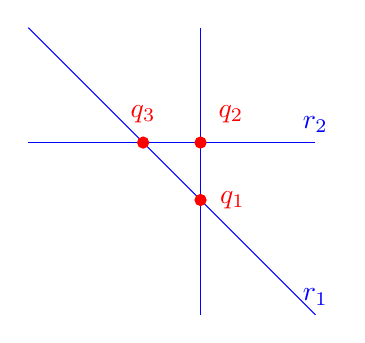
\begin{tikzpicture}
\begin{axis}[axis equal, hide axis,
        ticks=none,
        width=0.5*\linewidth,
        enlargelimits=0,
        axis lines=center,
        view={10}{20},
        ymin=-2,ymax=3,
        xmin=-2,xmax=3]

        \addplot [mark=*,color=red] coordinates {(1,0)} node[label=0:$q_1$]{};
        \addplot [mark=*,color=red] coordinates {(1,1)} node[label=50:$q_2$]{};
        \addplot [mark=*,color=red] coordinates {(0,1)} node[label=$q_3$]{};

        \draw (axis cs:-2,3) [color=blue] -- (axis cs:3,-2) node[above] {$r_1$};
        \draw (axis cs:-2,1) [color=blue] -- (axis cs:3,1) node[above] {$r_2$};
        \draw (axis cs:1,3) [color=blue] -- (axis cs:1,-2) node[label=310:$r_3$] {};

\end{axis}
\end{tikzpicture}
& \quad
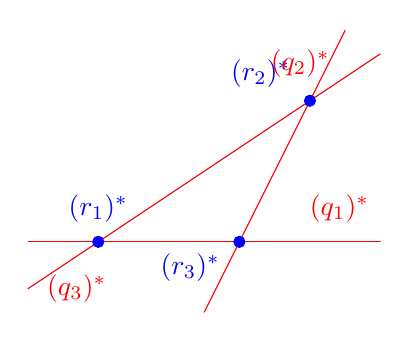
\begin{tikzpicture}
\begin{axis}[axis equal, hide axis,
        ticks=none,
        width=0.5*\linewidth,
        enlargelimits=0,
        axis lines=center,
        view={10}{20},
        ymin=0,ymax=4,
        xmin=0,xmax=5]

        \addplot [mark=*,color=blue] coordinates {(1,1)} node[label=$(r_1)^*$]{};
        \addplot [mark=*,color=blue] coordinates {(4,3)} node[label=160:$(r_2)^*$]{};
        \addplot [mark=*,color=blue] coordinates {(3,1)} node[label=190:$(r_3)^*$]{};

        \draw (axis cs:0,1) [color=red] -- (axis cs:5,1) node[label=100:$(q_1)^*$] {};
        \draw (axis cs:2.5,0) [color=red] -- (axis cs:4.5,4) node[label=240:$(q_2)^*$] {};
        \draw (axis cs:5,3.666) [color=red] -- (axis cs:0,0.333) node[label=0:$(q_3)^*$] {};

\end{axis}
\end{tikzpicture}
\end{aligned}
\]
\end{example}

\begin{example}
\[
\begin{aligned}
\text{Cuadrilátero en $\Po^2$} \qquad &\qquad \qquad\text{Cuadrilátero en $\left( \Po^2 \right)^*$} \\
\begin{tikzpicture}[line cap=round,line join=round,>=triangle 45,x=.8cm,y=.8cm]
\clip(2.,0.5) rectangle (8.5,7.);
\draw [line width=\pgflinewidth,color=blue,domain=2.:8.5] plot(\x,{(--4.-2.*\x)/-1.});
\draw [line width=\pgflinewidth,color=blue,domain=2.:8.5] plot(\x,{(--0.9088--0.7*\x)/1.24});
\draw [line width=\pgflinewidth,color=blue,domain=2.:8.5] plot(\x,{(--5.36-0.58*\x)/0.76});
\draw [line width=\pgflinewidth,color=blue,domain=2.:8.5] plot(\x,{(--15.4-1.88*\x)/1.});
\draw [line width=\pgflinewidth,dash pattern=on 2pt off 2pt,color=teal,domain=2.:8.5] plot(\x,{(--11.46-2.58*\x)/-0.24});
\draw [line width=\pgflinewidth,dash pattern=on 2pt off 2pt,color=teal,domain=2.:8.5] plot(\x,{(--14.942080928528313-1.2454296879136713*\x)/4.177002403922524});
\draw [line width=\pgflinewidth,dash pattern=on 2pt off 2pt,color=teal,domain=2.:8.5] plot(\x,{(--7.52--0.12*\x)/2.});
\begin{scriptsize}
\draw [fill=red] (4.,4.) circle (2.5pt);
\draw[color=red] (3.8004958677685994,4.598347107438018) node {$q_4$};
\draw [fill=red] (5.,6.) circle (2.5pt);
\draw[color=red] (5.35,6.135537190082645) node {$q_1$};
\draw [fill=red] (6.,4.12) circle (2.5pt);
\draw[color=red] (6.1806611570247965,4.647933884297522) node {$q_2$};
\draw [fill=red] (4.76,3.42) circle (2.5pt);
\draw[color=red] (5.23,3.44) node {$q_3$};
\draw[color=blue] (5.957520661157028,8.606611570247933) node {$f$};
\draw[color=blue] (-5.216033057851232,-1.8396694214875977) node {$g$};
\draw[color=blue] (-2.1747107438016466,9.0198347107438) node {$h$};
\draw[color=blue] (3.420330578512401,8.598347107438016) node {$r_1$};
\draw [fill=red] (3.2970786516853927,2.594157303370786) circle (2.5pt);
\draw[color=red] (3.1062809917355416,3.011570247933887) node {$q_5$};
\draw [fill=red] (7.4740810556079165,1.3487276154571146) circle (2.5pt);
\draw[color=red] (7.635206611570251,1.6892561983471108) node {$q_6$};
\draw[color=teal] (5.131074380165293,9.730578512396692) node {$j$};
\draw[color=teal] (-6.34,5.350413223140498) node {$k$};
\draw[color=teal] (-6.34,3.25123966942149) node {$l$};
\end{scriptsize}
\end{tikzpicture}
& \qquad
\begin{tikzpicture}[line cap=round,line join=round,>=triangle 45,x=.8cm,y=.8cm]
\clip(5.5,2.5) rectangle (12.,7.5);
\draw [line width=\pgflinewidth,color=red,domain=5.5:12.] plot(\x,{(--18.876--0.12*\x)/2.92});
\draw [line width=\pgflinewidth,color=red,domain=5.5:12.] plot(\x,{(--11.1072-1.32*\x)/-0.14});
\draw [line width=\pgflinewidth,color=red,domain=5.5:12.] plot(\x,{(-0.564--0.86*\x)/1.3});
\draw [line width=\pgflinewidth,color=red,domain=5.5:12.] plot(\x,{(-22.7588--2.06*\x)/-1.48});
\draw [line width=\pgflinewidth,color=red,domain=5.5:12.] plot(\x,{(--26.1456-1.2*\x)/2.78});
\draw [line width=\pgflinewidth,color=red,domain=5.5:12.] plot(\x,{(--10.0756-2.18*\x)/-1.44});
\begin{scriptsize}
\draw [fill=blue] (6.22,6.72) circle (2.5pt);
\draw[color=blue] (6.3,7.1) node {$r_1$};
\draw [fill=blue] (9.14,6.84) circle (2.5pt);
\draw[color=blue] (9.43,6.67) node {$r_4$};
\draw [fill=blue] (9.,5.52) circle (2.5pt);
\draw[color=blue] (9.27,5.1) node {$r_3$};
\draw [fill=blue] (7.7,4.66) circle (2.5pt);
\draw[color=blue] (7.55,5.32) node {$r_2$};
\draw[color=red] (-2.42,6.21) node {$f$};
\draw[color=red] (9.3,10.83) node {$g$};
\draw[color=red] (-2.42,-1.67) node {$h$};
\draw[color=red] (3.52,10.83) node {$i$};
\draw[color=red] (-2.42,10.31) node {$j$};
\draw[color=red] (11.48,10.83) node {$k$};
\draw [fill=teal] (8.753295272078507,3.193926851025867) circle (2.0pt);
\draw [fill=teal] (11.11824048913044,6.921297554347826) circle (2.0pt);
\draw [fill=teal] (8.4304647937959,5.765842535052128) circle (2.0pt);
\end{scriptsize}
\end{tikzpicture}
\end{aligned}
\]
\end{example}

\begin{defi}
Sea $\mathcal{R} = \setb{p_0,\dots,p_n;\overline{p}}$ una referencia de $\Po^n$, sea
$B = \setb{u_0,\dots,u_n}$ una base adaptada y sea $B^* = \setb{u_0^*,\dots,u_n^*}$
su base dual. Entonces, llamamos referencia dual de $\mathcal{R}$ a
\[
  \mathcal{R}^* = \setb{{p_0^\prime}=[u_0^*],\dots,{p_n^\prime}=[u_n^*];\overline{p}^\prime = [u_0^*+ \cdots + u_n^*]}
\]
\end{defi}

\begin{obs}
$\mathcal{R}^*$ no depende de la base $B$ escogida.
\end{obs}
\begin{example}
  En coordenadas, sea $p \in \Po^n$ y sea $p_\mathcal{R} = (a_0,\dots,a_n)$, entonces $p^*$
  es un hiperplano de $\left( \Po^n \right)^*$ y, en referencia $\mathcal{R}^*$ se tiene
  \[
    p^* \equiv a_0x_0^\prime + \cdots + a_nx_n^\prime = 0
  \]
  Y si $H \subseteq \Po^n$ en referencia $\mathcal{R}$
  \[
    \Po^n \supseteq H \equiv b_0x_0 + \cdots + b_nx_n = 0
  \]
  entonces $\left(H^*\right)_{\mathcal{R}^*} = (b_0,\dots,b_n)$
\end{example}

\begin{obs}
En general, si tenemos $\mathcal{R}$ una referencia de $\Po^n$ y
$\mathcal{R}^* = \setb{{p_0}^\prime,\dots,{p_n}^\prime; \overline{p}^\prime}$
una refencia de $\left( \Po^n \right)^*$. Entonces $\left( {p_i}^\prime \right)^*$
es un hiperplano tal que $p_i \notin \left( {p_i}^\prime \right)^*$ y
$p_j \in \left( {p_i}^\prime \right)^*$ $\forall i \neq j$
\end{obs}

%%%%%%%%%%%%%%%%%%%%
%   23 d'octubre   %
%%%%%%%%%%%%%%%%%%%%

\section{Los teoremas de Desargues y Pappus}

\begin{teo}[de Desargues]

Sean $ABC$, $A'B'C'$ dos triángulos en $\Po^2$ (sin vértices ni lados en común). Entonces,
\[
AA' \cap BB' \cap CC' \neq \emptyset \iff
\begin{cases}
AB \cap A'B' = Z \\
AC \cap A'C' = Y \\
BC \cap B'C' = X
\end{cases}
\text{ están alineados.}
\]

\begin{center}
\begin{tikzpicture}[line cap=round,line join=round,>=triangle 45,x=1.5cm,y=1.5cm]
\clip(-0.5,-0.5) rectangle (9.,3.5);
\fill[line width=\pgflinewidth,color=teal,fill=teal,fill opacity=0.10000000149011612] (3.3336552362849274,1.992339795349051) -- (1.9793647349081451,0.1168150700088304) -- (-0.19217003454083312,0.6438220176250907) -- cycle;
\fill[line width=\pgflinewidth,color=teal,fill=teal,fill opacity=0.10000000149011612] (4.403859447556563,2.040558909290155) -- (4.738313888759495,1.0095694436469795) -- (5.374944253774689,1.657128809689663) -- cycle;
\draw [line width=\pgflinewidth,color=teal] (3.3336552362849274,1.992339795349051)-- (1.9793647349081451,0.1168150700088304);
\draw [line width=\pgflinewidth,color=teal] (1.9793647349081451,0.1168150700088304)-- (-0.19217003454083312,0.6438220176250907);
\draw [line width=\pgflinewidth,color=teal] (-0.19217003454083312,0.6438220176250907)-- (3.3336552362849274,1.992339795349051);
\draw [line width=\pgflinewidth,color=teal] (4.403859447556563,2.040558909290155)-- (4.738313888759495,1.0095694436469795);
\draw [line width=\pgflinewidth,color=teal] (4.738313888759495,1.0095694436469795)-- (5.374944253774689,1.657128809689663);
\draw [line width=\pgflinewidth,color=teal] (5.374944253774689,1.657128809689663)-- (4.403859447556563,2.040558909290155);
\draw [line width=\pgflinewidth,dashed=on 3.pt off 3.pt,color=blue,domain=-0.5:9.] plot(\x,{(--3.6701280196078825-0.383430099600492*\x)/0.9710848062181263});
\draw [line width=\pgflinewidth,dashed=on 3.pt off 3.pt,color=blue,domain=-0.5:9.] plot(\x,{(--3.5541459610560944-1.8755247253402205*\x)/-1.3542905013767823});
\draw [line width=\pgflinewidth,dashed=on 3.pt off 3.pt,color=blue,domain=-0.5:9.] plot(\x,{(--5.2228066883522954-1.0309894656431755*\x)/0.334454441202932});
\draw [line width=\pgflinewidth,dashed=on 3.pt off 3.pt,color=blue,domain=-0.5:9.] plot(\x,{(--2.529148647580714--1.34851777772396*\x)/3.5258252708257607});
\draw [line width=\pgflinewidth,dashed=on 3.pt off 3.pt,color=blue,domain=-0.5:9.] plot(\x,{(-1.2968069532830016--0.5270069476162603*\x)/-2.171534769448978});
\draw [line width=\pgflinewidth,dashed=on 3.pt off 3.pt,color=blue,domain=-0.5:9.] plot(\x,{(-2.425616974499177--0.6475593660426835*\x)/0.6366303650151943});
\draw [line width=\pgflinewidth,color=gray,domain=-0.5:9.] plot(\x,{(--9.50601349361014--0.23250306512482055*\x)/5.1603138069701515});
\draw [line width=\pgflinewidth,color=gray,domain=-0.5:9.] plot(\x,{(--1.9667522247370517-1.215273416826892*\x)/-3.7556551544955843});
\draw [line width=\pgflinewidth,color=gray,domain=-0.5:9.] plot(\x,{(--2.1171944617344565--0.5677140507842084*\x)/3.11902478948039});
\draw [line width=\pgflinewidth,color=orange,domain=-0.5:9.] plot(\x,{(--2.855613634592153-0.8059659723881762*\x)/-0.14358796715525868});
\begin{scriptsize}
\draw [fill=purple] (8.49396904325508,2.2248428604738715) circle (2.5pt);
\draw[color=purple] (8.5756934700623,2.511596640794484) node {$O$};
\draw [fill=teal] (3.3336552362849274,1.992339795349051) circle (2.5pt);
\draw[color=teal] (3.1818813007858053,2.3100939843529726) node {$A$};
\draw [fill=teal] (-0.19217003454083312,0.6438220176250907) circle (2.5pt);
\draw[color=teal] (-0.1104456077336135,0.9305757979457029) node {$B$};
\draw [fill=teal] (1.9793647349081451,0.1168150700088304) circle (2.5pt);
\draw[color=teal] (1.8742904718702913,0.4500694633544068) node {$C$};
\draw [fill=teal] (4.403859447556563,2.040558909290155) circle (2.5pt);
\draw[color=teal] (4.52449688404727,2.3255941886946276) node {$A'$};
\draw [fill=teal] (4.738313888759495,1.0095694436469795) circle (2.5pt);
\draw[color=teal] (4.512821965931953,1.2250796804371424) node {$C'$};
\draw [fill=teal] (5.374944253774689,1.657128809689663) circle (2.5pt);
\draw[color=teal] (5.365090988350101,1.4265823368786539) node {$B'$};
\draw [fill=red] (4.082899471593713,3.029950328105273) circle (2.0pt);
\draw[color=red] (3.8006519608976106,3.1316048144606725) node {$Y$};
\draw [fill=red] (3.939311504438454,2.223984355717097) circle (2.0pt);
\draw[color=red] (3.8240017971282447,2.511596640794484) node {$Z$};
\draw [fill=red] (3.498235188833963,-0.2517976241139916) circle (2.0pt);
\draw[color=red] (3.3803549087461957,0.07806455915469361) node {$X$};
\draw[color=orange] (3.6,1) node {$r$};
\end{scriptsize}
\end{tikzpicture}
\end{center}

\end{teo}
\begin{proof}
$\implies$ Analítica \\
$R = \{A,B,C;O\}$, es un sistema de referencia porque todos los puntos son linealmente independientes.
\begin{itemize}
    \item $A,B,C$ linealmente independientes ($ABC$ triangulo)
    \item $A,B,O$ linealmente independientes (si no, $AB = A'B'$)
    \item $B,C,O$ linealmente independientes (si no, $BC = B'C'$)
    \item $C,A,O$ linealmente independientes (si no, $AC = A'C'$)
\end{itemize}
Tenemos que
\begin{itemize}
    \item $A' \in AO : x_1 - x_2 = 0$ i $A \neq A' \implies A' = (a:1:1)$
    \item $B' \in BO : x_0 - x_2 = 0$ i $B \neq B' \implies B' = (1:b:1)$
    \item $C' \in CO : x_0 - x_1 = 0$ i $C \neq C' \implies C' = (1:1:c)$
\end{itemize}

\begin{gather*}
Z : \left. \begin{cases}
AB : x_2 = 0 \\
A'B' : 0 = \begin{vmatrix} a & 1 & x_0 \\ 1 & b & x_1 \\ 1 & 1 & x_2 \end{vmatrix}
\end{cases} \right\}
x_0(1-b)-x_1(a-1)=x_0(1-b) + x_1(1-a) = 0 \implies \\ \implies Z = (a-1:1-b:0).
\end{gather*}
Análogamente, $X = (0:b-1:1-c), Y = (a-1:0:1-c)$. Vemos que $Z-X = Z \implies X,Y,Z$ no son linealmente independientes $\iff X,Y,Z$
están alineados. \\ \\
$\implies$ Sintética \\
$\overbrace{\Po^2 = \Po(\E)}^{\pi \text{ plano en } \Po^3} \subset \Po(\overline{\E}) = \Po^3, \overline{\E} = \E \times \k$ \\
Sea $r$ una recta en $\Po^3$, $r \nsubseteq \pi$, tal que $r \cap \pi = O$. Sean $p,p' \in r, p\neq p', p, p' \neq O$.
$r$ y $AA'$ son coplanarias $\implies pA \cap p'A' = A_0$ (intersección de rectas en un plano). Análogamente,
$\begin{cases} pB \cap p'B' = B_0 \\ pC \cap p'C' = C_0 \end{cases}$. \\
Por construcción,
\begin{align*}
    pA_0 \cap \pi &= A, & pB_0 \cap \pi &= B, & pC_0 \cap \pi = C \\
    p'A_0 \cap \pi &= A', & p'B_0 \cap \pi &= B', & p'C_0 \cap \pi = C'
\end{align*}
$A_0, B_0, C_0$ son linealmente independientes (forman un triángulo). Si estuvieran alineados, $T = A_0 \vee B_0 \vee C_0 \implies A,B,C \in
\pi \cap (p \vee t)$ estarían alineados.\\
Finalmente,
\begin{gather*}
    Z = AB \cap A'B'= \pi \cap \left( \left( A_0 \vee B_0 \vee p \right) \cap \left( A_0 \vee B_0 \vee p' \right) \right)
    \substack{\text{intersección de} \\ = \\ \text{planos distintos}} \pi \cap \left( A_0 \vee B_0 \right)
\end{gather*}
Análogamente, $Y = \pi \cap \left( A_0 \vee C_0 \right)$ y $X = \pi \cap \left( B_0 \vee C_0 \right)$. Entonces, $X,Y,Z \in \pi\cap\left(
A_0 \vee B_0 \vee C_0 \right)$ (que es una recta porque es la intersección de dos planos distintos).
\\ \\
$\impliedby$ Dualidad \\
Hipotésis: $X, Y, Z$ están alineados.

Consideramos el espacio proyectivo dual y dualizamos las hipótesis:

\begin{center}
\begin{tikzpicture}[line cap=round,line join=round,>=triangle 45,x=1.4cm,y=1.4cm]
\clip(-0.8,0.) rectangle (10.,4.5);
\fill[line width=\pgflinewidth,color=blue,fill=blue,fill opacity=0.10000000149011612] (3.5905034348218994,2.7363496037484754) -- (2.236212933445119,0.3958187481586135) -- (-0.36,0.52) -- cycle;
\fill[line width=\pgflinewidth,color=blue,fill=blue,fill opacity=0.10000000149011612] (4.564320062604457,2.6690117085413894) -- (4.909911174012507,1.1462661459359629) -- (5.7636405841417275,1.6921417570208015) -- cycle;
\draw [line width=\pgflinewidth,color=blue] (3.5905034348218994,2.7363496037484754)-- (2.236212933445119,0.3958187481586135);
\draw [line width=\pgflinewidth,color=blue] (2.236212933445119,0.3958187481586135)-- (-0.36,0.52);
\draw [line width=\pgflinewidth,color=blue] (-0.36,0.52)-- (3.5905034348218994,2.7363496037484754);
\draw [line width=\pgflinewidth,color=blue] (4.564320062604457,2.6690117085413894)-- (4.909911174012507,1.1462661459359629);
\draw [line width=\pgflinewidth,color=blue] (4.909911174012507,1.1462661459359629)-- (5.7636405841417275,1.6921417570208015);
\draw [line width=\pgflinewidth,color=blue] (5.7636405841417275,1.6921417570208015)-- (4.564320062604457,2.6690117085413894);
\draw [line width=\pgflinewidth,dashed=on 3.pt off 3.pt,color=teal,domain=-0.8:10.] plot(\x,{(--7.659747632557802-0.9768699515205879*\x)/1.1993205215372704});
\draw [line width=\pgflinewidth,dashed=on 3.pt off 3.pt,color=teal,domain=-0.8:10.] plot(\x,{(--4.697871799499361-2.340530855589862*\x)/-1.3542905013767803});
\draw [line width=\pgflinewidth,dashed=on 3.pt off 3.pt,color=teal,domain=-0.8:10.] plot(\x,{(--7.872684844357776-1.5227455626054265*\x)/0.34559111140804966});
\draw [line width=\pgflinewidth,dashed=on 3.pt off 3.pt,color=teal,domain=-0.8:10.] plot(\x,{(--2.852147643456839--2.2163496037484753*\x)/3.9505034348218993});
\draw [line width=\pgflinewidth,dashed=on 3.pt off 3.pt,color=teal,domain=-0.8:10.] plot(\x,{(-1.305325474728563--0.12418125184138651*\x)/-2.596212933445119});
\draw [line width=\pgflinewidth,dashed=on 3.pt off 3.pt,color=teal,domain=-0.8:10.] plot(\x,{(-1.70159964186535--0.5458756110848386*\x)/0.8537294101292208});
\draw [line width=\pgflinewidth,color=red,domain=-0.8:10.] plot(\x,{(--16.72573405137783-0.38750510854135545*\x)/5.603960695352214});
\draw [line width=\pgflinewidth,color=red,domain=-0.8:10.] plot(\x,{(--0.9933148705940678-1.202578349271157*\x)/-4.2845529561616065});
\draw [line width=\pgflinewidth,color=red,domain=-0.8:10.] plot(\x,{(--2.0204412296839145--0.6567027381863184*\x)/3.4308235460323857});
\draw [line width=\pgflinewidth,color=purple,domain=-0.8:10.] plot(\x,{(--3.193311356394389-0.8938251320959107*\x)/-0.1608060938655136});
\begin{scriptsize}
\draw [fill=orange] (9.194464130174113,2.34884449520712) circle (2.5pt);
\draw[color=orange] (9.276188556981314,2.55) node {$r^*$};
\draw [fill=blue] (3.5905034348218994,2.7363496037484754) circle (2.5pt);
\draw[color=blue] (3.78,2.55) node {\tiny $(AB)^*$};
\draw [fill=blue] (-0.36,0.52) circle (2.5pt);
\draw[color=blue] (-0.4,0.7) node {\tiny $(AC)^*$};
\draw [fill=blue] (2.236212933445119,0.3958187481586135) circle (2.5pt);
\draw[color=blue] (2.1,0.6) node {\tiny $(BC)^*$};
\draw [fill=blue] (4.564320062604457,2.6690117085413894) circle (2.5pt);
\draw[color=blue] (4.95,2.85) node {\tiny $(A'B')^*$};
\draw [fill=blue] (4.909911174012507,1.1462661459359629) circle (2.5pt);
\draw[color=blue] (5.3,1.05) node {\tiny $(B'C')^*$};
\draw [fill=blue] (5.7636405841417275,1.6921417570208015) circle (2.5pt);
\draw[color=blue] (5.84,1.93) node {\tiny $(A'C')^*$};
\draw[color=blue] (2.7966090029803388,1.76) node {\tiny $(B)^*$};
\draw[color=blue] (0.9753217769908749,0.35) node {\tiny $(C)^*$};
\draw[color=blue] (1.7225165363711676,1.48) node {\tiny $(A)^*$};
\draw[color=blue] (4.5,1.75) node {\tiny $(B')^*$};
\draw[color=blue] (5.61,1.3955819281953425) node {\tiny $(C')^*$};
\draw[color=blue] (5.330066234004144,2.3410943930362804) node {\tiny $(A')^*$};
\draw [fill=gray] (4.278993131711778,3.926220888888763) circle (2.0pt);
\draw[color=gray] (4.7,3.9531156445683706) node {\tiny $(BB')^*$};
\draw [fill=gray] (4.118187037846265,3.032395756792852) circle (2.0pt);
\draw[color=gray] (3.78,3.02) node {\tiny $(AA')^*$};
\draw [fill=gray] (3.631836574987902,0.32906371097595916) circle (2.0pt);
\draw[color=gray] (3.38,0.5) node {\tiny $(CC')^*$};
\draw[color=red] (7.6,2.57) node {$Z^*$};
\draw[color=red] (7.209728050570193,2.1) node {$Y^*$};
\draw[color=red] (7.443226412876534,1.7) node {$X^*$};
\draw[color=purple] (4.17,2.186092349619733) node {$O^*$};
\end{scriptsize}
\end{tikzpicture}
\end{center}

Queremos ver que, en efecto, $\left(AA'\right)^*, \left(BB'\right)^*, \left(CC'\right)^*$ están alineados. Por la primera implicación,
$\exists s \subset (\Po^2)^*$ recta tal que:

\begin{align*}
    s &= \left[ \left[ \left(AB\right)^* \vee \left(AC\right)^* \right] \cap \left[ \left(A'B'\right)^* \vee \left(A'C'\right)^* \right] \right]
    \vee [\dots ] \vee [\dots] \\
    &= \left[ (AB \cap AC)^* \cap \left(A'B' \cap A'C' \right)^* \right] \vee [\dots] \vee [\dots] \\
    &= \left(A^* \cap (A')^* \right) \vee \left(B^* \cap (B')^* \right) \vee \left(C^* \cap (C')^* \right) \\
    &= (AA')^* \vee (BB')^* \vee (CC')^*
\end{align*}

$s = (AA' \cap BB' \cap CC')^* \implies AA' \cap BB' \cap CC' = s^*$ (un punto)
\end{proof}
\begin{obs}
El teorema de Desargues es su propio dual: $(\implies) \iff (\impliedby)$.
\end{obs}
\begin{obs}
Definición axiomática de $\Po^2$
\begin{itemize}
    \item $X \rightarrow$ puntos
    \item $Y \rightarrow$ rectas
\end{itemize}
Hay una relación de pertenencia entre puntos y rectas (los puntos pertenecen a rectas). Axiomas:
\begin{itemize}
    \item $\forall p_1, p_2, \exists! r$ tal que $p_1, p_2 \in r$
    \item $\forall r_1, r_2, \exists! p$ tal que $p \in r_1, r_2$
    \item $\exists 4$ puntos no alineados
\end{itemize}
\end{obs}

%%%%%%%%%%%%%%%%%
% 25 de OCTUBRE %
%%%%%%%%%%%%%%%%%

\begin{teo}[ de Pappus]
Sean $r,s \subseteq \Po^2_\k$ rectas diferentes ($r \neq s$), sean
$A,B,C \in r$ tal que $A \neq B$, $B \neq C$ y $C\neq A$ y sean también
$A^\prime,B^\prime,C^\prime \in s$ tal que $A^\prime \neq B^\prime$,
$B^\prime \neq C^\prime$ y $C^\prime \neq A^\prime$. Entonces
$x_0 \equiv AB^\prime \cap A^\prime B$, $x_1 \equiv AC^\prime \cap A^\prime C$
y $x_2 \equiv BC^\prime \cap B^\prime C$ están alineados.
\end{teo}

\begin{proof}
\begin{itemize}
    \item[]
\end{itemize}
\begin{center}
\begin{tikzpicture}[line cap=round,line join=round,>=triangle 45,x=1.0cm,y=1.0cm]
\clip(0.,1.) rectangle (16.,6.5);
\draw [line width=\pgflinewidth,domain=0.:16.] plot(\x,{(--79.6976-2.26*\x)/13.74});
\draw [line width=\pgflinewidth,domain=0.:16.] plot(\x,{(-14.3512-1.36*\x)/-10.5});
\draw [line width=\pgflinewidth,dashed=on 3.pt off 3.pt,color=red,domain=0.:16.] plot(\x,{(--26.092656187893812-3.6181394152023674*\x)/3.9761421876856913});
\draw [line width=\pgflinewidth,dashed=on 3.pt off 3.pt,color=blue,domain=0.:16.] plot(\x,{(--42.70862317344715-3.2268316852907533*\x)/6.997268043620948});
\draw [line width=\pgflinewidth,dashed=on 3.pt off 3.pt,color=red,domain=0.:16.] plot(\x,{(--6.74835353562346-3.3609489282203526*\x)/-1.5278748314441364});
\draw [line width=\pgflinewidth,dashed=on 3.pt off 3.pt,color=green,domain=0.:16.] plot(\x,{(--30.41940935288539-2.6841105452109573*\x)/3.697715625613694});
\draw [line width=\pgflinewidth,dashed=on 3.pt off 3.pt,color=green,domain=0.:16.] plot(\x,{(--8.1210274102988-2.575916771217369*\x)/-2.360202559373546});
\draw [line width=\pgflinewidth,dashed=on 3.pt off 3.pt,color=blue,domain=0.:16.] plot(\x,{(--0.10340002392072734-2.86144742431515*\x)/-4.5646671604961195});
\draw [line width=\pgflinewidth,color=orange,domain=0.:16.] plot(\x,{(--6.478551211506101--0.15741244291993972*\x)/2.100043160860284});
\begin{scriptsize}
\draw [fill=purple] (15.08,3.32) circle (2.5pt);
\draw[color=purple] (15.27,3.74) node {$O$};
\draw [fill=purple] (1.0220234435922084,5.63230182077741) circle (2.5pt);
\draw[color=purple] (1.16,6.01) node {$A$};
\draw [fill=purple] (4.321575861599462,5.089580680697614) circle (2.5pt);
\draw[color=purple] (4.26,5.45) node {$B$};
\draw [fill=purple] (7.358368190651445,4.590079176792411) circle (2.5pt);
\draw[color=purple] (7.5,4.97) node {$C$};
\draw [fill=purple] (2.793701030155326,1.728631752477261) circle (2.5pt);
\draw[color=purple] (2.8,2.09) node {$A'$};
\draw [fill=purple] (4.9981656312778995,2.0141624055750422) circle (2.5pt);
\draw[color=purple] (5.2,2.39) node {$B'$};
\draw [fill=purple] (8.019291487213156,2.4054701354866563) circle (2.5pt);
\draw[color=purple] (8.22,2.77) node {$C'$};

\draw [fill=orange] (6.420232165913115,3.566200819314453) circle (2.0pt);
\draw[color=orange] (6.56,3.89) node {$x_2$};
\draw [fill=orange] (5.630631420487521,3.507014901336497) circle (2.0pt);
\draw[color=orange] (5.78,3.83) node {$x_1$};
\draw [fill=orange] (3.5305882596272373,3.349602458416557) circle (2.0pt);
\draw[color=orange] (3.5,3.67) node {$x_0$};
\end{scriptsize}
\end{tikzpicture}
\end{center}

Tomamos la referencia $\mathcal{R} = \setb{A,B,A^\prime;B^\prime}$. Entonces
\[
\begin{aligned}
A = (1,0,0) &\qquad A^\prime = (0,0,1) \\
B = (0,1,0) &\qquad B^\prime = (1,1,1) \\
C = (1,a,0) &\qquad C^\prime = (1,1,b)
\end{aligned}
\]
con $a,b \neq 0$. Calculamos ahora $x_0$, $x_1$ y $x_
2$ y vemos que
\[
  \determinant{\line(1,0){25} & x_0 & \line(1,0){25} \\
    \line(1,0){25} & x_1 & \line(1,0){25} \\ \line(1,0){25} & x_2 & \line(1,0){25}} = 0
\]
\end{proof}


\section{Coordenadas absolutas. Razón doble}

\begin{defi}
  Sea $\R = \setb{p_0,p_1;\overline{p}}$ un sistema de referencia de $\Po^1_\k$ y
  sea $q \in \Po^1_k$ con $q_\R = (x_0,x_1)$ las coordenadas de $q$ en la
  referencia $\R$. Definimos las coordenas absolutas de $q$ como
  \[
    \alpha = \frac{x_0}{x_1} \in k \cup \setb{\infty}
  \]
\end{defi}

\begin{obs}
  A diferencia de las coordenadas normales, \textbf{NO} está definido salvo constantes.
\end{obs}
\begin{obs}
  Al trabajar con coordenadas absolutas, trabajaremos con aritmética normal de $0/\infty$.
\end{obs}
\begin{obs}
  \[
    \begin{aligned}
      \left( p_0 \right)_\R = (1,0) &\qquad \alpha_0 = \infty \\
      \left( p_1 \right)_\R = (0,1) &\qquad \alpha_1 = 0 \\
      \left( p_2 \right)_\R = (1,1) &\qquad \alpha_2 = 1 \\
    \end{aligned}
  \]
\end{obs}

\begin{defi}
  Sean $q_1, q_2, q_3, q_4 \in \Po^1_\k$ con al menos 3 de ellos diferentes. Sea
  $\R$ un sistema de referencia y sean $\left( q_i \right)_\R = (x_i:y_i)$
  $\forall i=1,2,3,4$. Definimos la razón doble de $q_1,q_2,q_3,q_4$ como
  \[
    \left( q_1,q_2,q_3,q_4 \right) = \frac{\determinant{x_3 & y_3 \\ x_1 & y_1}}
    {\determinant{x_3 & y_3 \\ x_2 & y_2}}:\frac{\determinant{x_4 & y_4 \\ x_1 & y_1}}
    {\determinant{x_4 & y_4 \\ x_2 & y_2}} \in k \cup \setb{\infty}
  \]
\end{defi}
\begin{obs}
  La razón doble no depende del sistema de referencia ni del representante
  de cada punto. De hecho, sean $\R$ y $\overline{\R}$ dos sistemas de referencia
  y $q_i = (x_i, y_i)_\R = (\overline{x}_i, \overline{y}_i)_{\overline{\R}}$, por lo tanto
  \[
    \begin{pmatrix} \overline{x}_i \\ \overline{y}_i \end{pmatrix} = S \begin{pmatrix}
      x_i \\ y_i \end{pmatrix}
  \]
  y se tiene que
  \[
    \frac{\determinant{\overline{x}_3 & \overline{y}_3 \\ \overline{x}_1 & \overline{y_1}}}
    {\determinant{\overline{x}_3 & \overline{y}_3 \\ \overline{x}_2 & \overline{y_2}}}:
    \frac{\determinant{\overline{x}_4 & \overline{y}_4 \\ \overline{x}_1 & \overline{y_1}}}
    {\determinant{\overline{x}_4 & \overline{y}_4 \\ \overline{x}_2 & \overline{y_2}}}
    =
    \frac{\cancel{\det S}\determinant{x_3 & y_3 \\ x_1 & y_1}}
    {\cancel{\det S} \determinant{x_3 & y_3 \\ x_2 & y_2}}:
    \frac{\cancel{\det S} \determinant{x_4 & y_4 \\ x_1 & y_1}}
    {\cancel{\det S} \determinant{x_4 & y_4 \\ x_2 & y_2}}
  \]
\end{obs}
\begin{obs}
  La razón doble es cociente de razones simples
\end{obs}
\begin{obs}
  En coordenadas absolutas, si
  \[
    \begin{aligned}
      q_1 &\qquad \alpha_1 &\qquad (\alpha_1:1) \\
      q_2 &\qquad \alpha_2 &\qquad (\alpha_2:1) \\
      q_3 &\qquad \alpha_3 &\qquad (\alpha_3:1) \\
      q_4 &\qquad \alpha_4 &\qquad (\alpha_4:1) \\
    \end{aligned}
  \]
  teniendo en cuenta que $(\infty,1) = (1,0)$. emtonces,
  \[
    \left( q_1,q_2,q_3,q_4 \right) = \frac{\determinant{\alpha_3 & 1 \\ \alpha_1 & 1}}
    {\determinant{\alpha_3 & 1 \\ \alpha_2 & 1}}:\frac{\determinant{\alpha_4 & 1 \\ \alpha_1 & 1}}
    {\determinant{\alpha_4 & 1 \\ \alpha_2 & 1}} =
    \frac{\alpha_3-\alpha_1}{\alpha_3-\alpha_2}:\frac{\alpha_4-\alpha_1}{\alpha_4-\alpha_2}
  \]
\end{obs}
\begin{obs}\label{obs:rzdo_ref}
  Sean $q_1,q_2,q_3,q_4 \in \Po^1_\k$ tal que $\setb{q_1,q_2,q_3}$ son diferentes dos a dos.
  Tomamos $\R = \setb{q_1,q_2;q_3}$ como nuestro sistema de referencia y sean $(x,y)_\R = q_4$
  las coordenadas de $q_4$ en el sistema de referencia $\R$, entonces
  \[
    \left( q_1,q_2,q_3,q_4 \right) = \frac{\determinant{1 & 1 \\ 1 & 0}}
    {\determinant{1 & 1 \\ 0 & 1}}:\frac{\determinant{x & y \\ 1 & 0}}
    {\determinant{x & y \\ 0 & 1}} = \frac{-1}{1}:\frac{-y}{x} = \frac{x}{y}
  \]
  es decir, la coordenada absoluta de $q_4$ en la referencia $\R = \setb{q_1,q_2;q_3}$.
\end{obs}
\begin{obs}
 Sea $V \subseteq \Po^n$ una variedad de dimensión $n-2$, por lo tanto $V^*$ es una recta de
 $\left( \Po^n \right)^*$ y si $V \subseteq H_1,H_2,H_3,H_4 \subseteq \Po^n$, la razón doble
 de $H_1,H_2,H_3,H_4$ queda definida considerando los hiperplanos como puntos del espacio dual,
 es decir,
 \[
  (H_1,H_2,H_3,H_4) = (H_1^*,H_2^*,H_3^*,H_4^*)
 \]
\end{obs}

\begin{example}
 Consideramos $V \subseteq \Po^4$
 \[
  V : \begin{cases}
       x_0 = 0 \\ x_1 = 0
      \end{cases}
 \]
 Podemos identificar $V^* = \setb{H^* \in \left( \Po^4 \right)^* \text{ hiperplano } \vert V \subseteq H}$.
 Tomamos ahora
 \[
  \begin{aligned}
   H_1 &\rightarrow x_0 = 0 &\leftrightarrow (1,0,0,0) \\
   H_2 &\rightarrow x_1 = 0 &\leftrightarrow (0,1,0,0) \\
   H_3 &\rightarrow 2x_0+x_1 = 0 &\leftrightarrow (2,1,0,0) \\
   H_4 &\rightarrow 3x_0+2x_1 = 0 &\leftrightarrow (3,2,0,0)
  \end{aligned}
 \]
 Para calcular la razón doble, aplicamos la observación \ref{obs:rzdo_ref}, y tomamos el sistema
 de referencia $\R = \setb{H_1,H_2;H_3}$ y $B = \setb{(2,0,0,0),(0,1,0,0)}$ una base adaptada.
 Entonces se tiene que $\left( H_4 \right)_\R = \left( \frac{3}{2}, 2 \right) = (3,4)$. Por lo
 tanto,
 \[
  (H_1,H_2,H_3,H_4) = \frac{3}{4}
 \]
\end{example}

\begin{prop}
 Sean $q_1,q_2,q_3,q_4 \in \Po^n$ y sea $\rho = (q_1,q_2,q_3,q_4)$. Si permutamos los cuatro
 puntos, (con $4! = 24$ posiblidades), obtendremos uno de los sisguientes valores para la
 razón doble
 \[
   A_p = \setb{\rho, \frac{\rho}{1}, 1-\rho, \frac{1}{1-\rho}, \frac{\rho}{\rho-1}, \frac{\rho-1}{\rho}}
 \]

\end{prop}

%%%%%%%%%%%%%%%%%
% 27 de octubre %
%%%%%%%%%%%%%%%%%

\begin{defi}[Proyección y sección]
 Sean $V,r \subseteq \Po^n$ dos variedades suplementarias con $\dim r = 1$ ($\implies \dim V = n-2$).
 Entonces, definimos la proyección desde $V$ como
 \[
  \begin{aligned}
   \Phi \colon r &\to V^* \\ p &\mapsto V \vee p
  \end{aligned}
 \]
 De nuevo identificando los hiperplanos de $\Po^n$ con puntos de $\left( \Po^n \right)^*$. Asimismo,
 definimos la sección con $r$ como
 \[
  \begin{aligned}
   \Psi \colon V^* &\to r \\ H &\mapsto H \cap r
  \end{aligned}
 \]
\end{defi}

\begin{obs}
 $p \notin V \implies V \vee p$ es un hiperplano que contiene a $V$.
\end{obs}
\begin{obs}
 $\Psi$ está bien definido y $r \cap H$ es un punto. En efecto, si $r \cap H$ no es un punto,
 $r \subseteq H$, pero si nos miramos ahora $H \cong \Po^{n-1}$, entonces $V$ es un hiperplano
 de $H$, $\implies r \cap V \neq \emptyset$, lo cual es una contradicción ya que hemos supuesto que
 $V$ y $r$ son suplementarias.
\end{obs}
\begin{obs}
 $\Phi(\Psi(H)) = H$ y $\Psi(\Phi(p)) = p$, esd decir, $\Phi$ y $\Psi$ son inversas mutuas.
\end{obs}

\begin{teo}[de la invariancia de razón doble]
 Sean $V,r \subseteq \Po^n$ dos variades suplementarias con $\dim r = 1$ ($\implies \dim V = n-2$) y
 sean $\Phi$ y $\Psi$ la proyección desde $V$ y la sección con $r$ respectivamente. Entonces,
 \begin{enumerate}[i)]
  \item \label{item:teo_inv_1} $\forall p_1,p_2,p_3,p_4 \in r$ con $p_1,p_2,p_3$ distintos dos a dos
    \[
     (p_1,p_2,p_3,p_4) = \left( \Phi(p_1), \Phi(p_2), \Phi(p_3), \Phi(p_4) \right)
    \]
  \item \label{item:teo_inv_2} $\forall H_1,H_2,H_3,H_4 \in V^*$ (identificando hiperplanos con elementos del dual) con
  $H_1,H_2,H_3$ distintos dos a dos. Entonces
    \[
     (H_1,H_2,H_3,H_4) = \left( \Psi(H_1), \Psi(H_2), \Psi(H_3), \Psi(H_4) \right)
    \]
 \end{enumerate}
 \label{teo:inv_rz_do}
\end{teo}

\begin{proof}
 Primero vemos que $\ref{item:teo_inv_1} \iff \ref{item:teo_inv_2}$ porque $\Psi^{-1}=\Phi$. Pasamos ahora
 a demostrar $\ref{item:teo_inv_1}$. Sea $\rho = (p_1,p_2,p_3,p_4)$, entonces podemos elegir $u_1,u_2 \in \E$
 tal que $p_1 = [u_1]$, $p_2=[u_2]$ y $p_3=[u_1+u_2]$. Por lo tanto $p_4 = [\rho u_1+u_2]$, de la misma forma,
 $\overline{\rho} = (H_1,H_2,H_3,H_4)$ y podemos escoger $w_1,w_2 \in \E^*$ tal que $H_1 = [w_1]$, $H_2 = [w_2]$ y
 $H_3=[w_1+w_2]$. Lo que implica que $H_4 = [\overline{\rho} w_1 + w_2]$. Ahora trabajamos con que $p_i \in H_i$.
 Entonces
 \[
  \begin{cases}
    p_1 \in H_1 \implies w_1(u_1) = 0 \\
    p_2 \in H_2 \implies w_2(u_2) = 0 \\
    p_3 \in H_3 \implies (w_1+w_2)(u_1+u_2) = 0 \implies \cancelto{0}{w_1(u_1)} + w_1(u2) + w_2(u_1) + \cancelto{0}{w_2(u_2)} = 0 \\
    p_4 \in H_4 \implies (\overline{\rho}w_1+w_2)(\rho u_1+u_2) = 0 \implies \cancelto{0}{\overline{\rho}w_1(u_1)} + \overline{\rho}w_1(u_2) +
      \rho w_2(u_1) + \cancelto{0}{w_2(u_2)} = 0
  \end{cases}
 \]
 trabajando ahora con la cuarta ecuación
 \[
  \overline{\rho}w_1(u_2) + \rho w_2(u_1) = w_1(u_2)(\overline{\rho} - \rho) = 0 \stackrel{(1)}{\implies} \overline{\rho} = \rho
 \]
 La cancelación en (1) ocurre ya que $w_1(u_2) \neq 0$. Y $w_1(u_2) \neq 0$ ya que, si lo fuera,
 \[
  w_1(u_2) = 0 \implies p_2 \in H_1 \implies \setb{p_1,p_2} \subseteq r \cap H_1 \implies r \subseteq H_1 \implies r \cap V \neq \emptyset
 \]
 pero como sabemos $r \cap V = \emptyset$ ya que son variedades suplementarias.
\end{proof}

\section{Cuaternas armónicas}

\begin{obs}
 Sean $p_1,p_2,p_3,p_4 \in \Po^n$ diferentes dos a dos. y sea
 \[
  A_p = \setb{\rho, \frac{1}{\rho}, 1-\rho, \frac{1}{1-\rho}, \frac{\rho}{\rho-1},\frac{\rho-1}{\rho}}
 \]
 Entonces, los valores de $A_p$ son diferentes, salvo el caso en que
 \[
  A_p = \setb{-1,\frac{1}{2},2} \qquad \text{con $\k = \real$}
 \]
\end{obs}

\begin{defi}
 Sean $p_1,p_2,p_3,p_4 \in \Po^n$ diferentes dos a dos. Entonces $\setb{p_1,p_2,p_3,p_4}$ forman
 una cuaterna armónica si y solo si
 \[
  (p_1,p_2,p_3,p_4) = -1
 \]
\end{defi}

\begin{prop}\label{prop:intercambio_raz_do}
 Sean $p_1,p_2,p_3,p_4 \in \Po^n$ diferentes dos a dos. Entonces, son eqivalentes
 \begin{enumerate}[i)]
  \item $\rho = (p_1,p_2,p_3,p_4) = -1$
  \item $(p_1,p_2,p_3,p_4) = (p_2,p_1,p_3,p_4)$
  \item $(p_1,p_2,p_3,p_4) = (p_1,p_2,p_4,p_3)$
  \item $(p_1,p_2,p_3,p_4) = (p_3,p_4,p_1,p_2)$
 \end{enumerate}
\end{prop}

%TODO hacer esta demo
\begin{proof}
 La demostración se hará en clase de problemas
\end{proof}

\begin{teo}[de la cuaterna armónica en el cuadrilátero]
 Sean $A,B,C,D,p_1,p_2 \in \Po^2$ los vértices de un cuadrilátero, sea $p_1p_2 = r \subseteq \Po^2$,
 $AC = s \subseteq \Po^2$, $s \cap BD = O \in \Po^2$, $s \cap r = p_3 \in \Po^2$ y $DB \cap r = p_4 \in \Po^2$.
 Entonces, $\setb{p_1,p_2,p_3,p_4}$ son una cuaterna armónica. Dicho de otra forma, en un cuadrilátero, la intersección
 de una diagonal con las otras dos y los vértices de la diagonal forman una cuaterna armónica.
    \begin{center}
        \begin{tikzpicture}[line cap=round,line join=round,>=triangle 45,x=0.7cm,y=0.7cm]
        \clip(-0.4,-10.4) rectangle (22.,-3.3);
        \draw [line width=\pgflinewidth,color=red,domain=-0.4:22.] plot(\x,{(-35.22799973025435-1.3294355912181954*\x)/6.229849702347544});
        \draw [line width=\pgflinewidth,color=red,domain=-0.4:22.] plot(\x,{(-84.60760112764035--4.830564408781805*\x)/8.489849702347545});
        \draw [line width=\pgflinewidth,color=red,domain=-0.4:22.] plot(\x,{(-9.366982581363288--1.2589742508617139*\x)/-0.663403814185445});
        \draw [line width=\pgflinewidth,color=red,domain=-0.4:22.] plot(\x,{(--33.09616283070619-0.8807667544560287*\x)/-3.382144337111148});
        \draw [line width=\pgflinewidth,color=orange,domain=-0.4:22.] plot(\x,{(-108.33231529321682--1.4734909227583532*\x)/11.156070080886488});
        \draw [line width=\pgflinewidth,color=orange,domain=-0.4:22.] plot(\x,{(-34.929545144732934--3.1050034233737476*\x)/1.0457864758935198});
        \draw [line width=\pgflinewidth,color=orange,domain=-0.4:22.] plot(\x,{(-37.6337145915516-0.07046134035648155*\x)/5.566445888162099});
        \begin{scriptsize}
        \draw [fill=blue] (9.764063698503698,-4.410167889099014) circle (2.0pt);
        \draw[color=blue] (10.01967608046732,-3.826713320136143) node {$A$};
        \draw [fill=blue] (11.076596185814555,-6.901025749138286) circle (2.5pt);
        \draw[color=blue] (11.323210877062243,-6.257629562434783) node {$B$};
        \draw [fill=blue] (8.718277222610178,-7.515171312472762) circle (2.0pt);
        \draw[color=blue] (9.13890932601129,-7.1383963168908116) node {$C$};
        \draw [fill=blue] (5.510150297652456,-6.830564408781805) circle (2.5pt);
        \draw[color=blue] (5.756764988900144,-6.1871682220783) node {$D$};
        \draw [fill=green] (8.934259258114592,-6.87390756018006) circle (2.0pt);
        \draw[color=green] (8.6,-6.6) node {$O$};
        \draw [fill=blue] (0.5839299191135113,-9.633490922758353) circle (2.0pt);
        \draw[color=blue] (0.912547839391988,-8.95277583107023) node {$p_1$};
        \draw [fill=blue] (11.74,-8.16) circle (2.5pt);
        \draw[color=blue] (12.080670285894428,-7.40262634322762) node {$p_2$};
        \draw [fill=green] (8.350302560934376,-8.607710382880954) circle (2.0pt);
        \draw[color=green] (8.9,-8.1) node {$p_3$};
        \draw [fill=green] (20.380280676850695,-7.018793907252667) circle (2.0pt);
        \draw[color=green] (20.712184479563508,-6.6) node {$p_4$};
        \end{scriptsize}
        \end{tikzpicture}
    \end{center}
\end{teo}

\begin{proof}
 Podemos poner poner coordemadas y operar y nos saldrá el resultado. Aunque aquí detallamos una demostración
 sintética. Para esta demostración nos valdremos de las proyecciones y secciones definidas anteriormente, por
 ello, recordamos que si $h \subseteq \Po^2$ es una recta, una variedad complementaria de $h$ es un punto. Ahora
 definimos $\Phi_B$ la proyección desde $B$, $\Phi_D$ la proyección desde $D$ y $\Psi_s$ y $\Psi_r$ la sección
 con $r$ y con $s$ respectivamente. entonces
 \[
  \begin{array}{ccc}
   r & \stackrel{\Psi_s \circ \Phi_B}{\to} s & \stackrel{\Psi_r \circ \Phi_D}{\to} r \\
   p_1 &\mapsto C &\mapsto p_2 \\
   p_2 &\mapsto A &\mapsto p_1 \\
   p_3 &\mapsto p_3 &\mapsto p_3 \\
   p_4 &\mapsto O &\mapsto p_4
  \end{array}
 \]
 Por el teorema \ref{teo:inv_rz_do}, tenemos que, si $f = \Psi_r \circ \Phi_D \circ \Psi_s \circ \Phi_B$,
 \[
  (p_1,p_2,p_3,p_4) = \left( f(p_1), f(p_2), f(p_3), f(p_4) \right) = (p_2,p_1,p_3,p_4)
 \]
 Y por la proposición \ref{prop:intercambio_raz_do}, tenemos que $\setb{p_1,p_2,p_3,p_4}$ es una cuaterna
 armónica.
\end{proof}


\section{Relación entre el espacio proyectivo y el afín}

%TODO cambio a recordatorio?
\begin{obs}
  Sea $\F$ un $\k$-e.v. de $\dim n$. Llamamos espacio afín de dimensión $n$ a
  $\A^n = \lp \A,\, \F,\, \delta \rp$ donde $\delta$ es una aplicación de la forma
  \[
    \begin{aligned}
      \delta \colon \A \times \A & \to \F  \\
      p,\, q &\mapsto \delta (p, q) = q - p = \overrightarrow{pq}
    \end{aligned}
  \]
  que cumple
  \begin{enumerate}[i)]
    \item 
      \[
        \begin{aligned}
          \delta_p \colon \A & \to \F  \\
          q &\mapsto \delta (p, q)
        \end{aligned}
        \text{ es biyectiva } \forall p \in \A.
      \]
    \item \[\delta(p, q) + \delta(q, r) = \delta(p,r) \qquad \forall p, q, r \in \A\].
  \end{enumerate}
\end{obs}

\subsection{Completación proyectiva del espacio afín $\A^n$}

\begin{defi}
  Sea $\F$ un $k$-e.v. de $\dim n$ asociado a $\A^n$ un espacio afín. Consideramos
  el espacio vectorial $\E = \k \times \F$, de manera que todo $v \in \E$ se puede 
  escribir como $v = \lp \alpha, \, \vec{\omega} \rp$, con $\alpha \in \k, \, 
  \vec{\omega} \in \F$. Entonces decimos que
  \begin{enumerate}[i)]
    \item $e_0 = \lp1, \vec{0}\rp.$
    \item Si $u \in \F, \, u = \lp 0, u \rp \in \E.$
  \end{enumerate}
\end{defi}

\begin{obs}
  En el espacio vectorial $\E$ construido en la definición anterior,
  podemos considerar 2 s.e.v., la recta $[e_0] \subseteq \E$ y el hiperplano
  $\{0\} \times \F \subseteq \E$. Con la notación definida anteriormente,
  tenemos $E = [e_0] \oplus \F$.
\end{obs}

\begin{defi}
  Con las mismas hipótesis y con el mismo espacio $\E$ que en la última definición,
  \begin{enumerate}[i)]
    \item $\Po^n = \Po (\E) = \overline{\A^n}$ es la completación proyectiva
    de $\A^n$.
    \item $\A^n_\infty = \pi(\F)$ son los puntos del infinito de $\A^n$.
  \end{enumerate}
\end{defi}

\begin{defi}
  Fijado $p_0 \in \A^n$, definimos
   \[
     \begin{aligned}
       \varphi \colon \A^n &\to \Po^n = \Po(\E)\\
       p &\mapsto \varphi(p) \coloneqq [e_0 + \overrightarrow{p_0p}]
     \end{aligned}
   \]
\end{defi}

%TODO aqui es pot fer un dibuix per il·lustrarho
\begin{obs}
  La idea detrás de esta función es asociar a todo punto en el afín una dirección
  en un espacio vectorial, situando el plano afín como un hiperplano 
  en un espacio vectorial de una dimensión más sin contener el origen, 
  y asignando a un punto afín la dirección que representa el vector entre el origen
  y el punto (considerados en el espacio vectorial).
\end{obs}

\begin{prop}
  \begin{enumerate}[i)]
    \item[]
    \item $\varphi$ es inyectiva.
    \item $\im \varphi = \Po^n \setminus \A^n_\infty$
  \end{enumerate}
\end{prop}

\begin{proof}
  \begin{enumerate}[i)]
    \item[]
    \item Supongamos $\varphi(p_1) = \varphi(p_2)$. Entonces
    \[
      [e_0 + \overrightarrow{p_0p_1}] = [e_0+\overrightarrow{p_0p_2}]
      \implies \exists \lambda \neq 0 \text{ t.q. } e_0 + \overrightarrow{p_0p_1}
      = \lambda e_0 + \lambda \overrightarrow{p_0p_2}
    \]
    Como $\E = [e_0] \oplus \F$
    \[e_0 = \lambda e_0 \implies \lambda = 1 \implies \overrightarrow{p_0p_1}
    = \lambda \overrightarrow{p_0p_2} = \overrightarrow{p_0p_2} \implies
    p_1 = p_2.\]
    Es decir, $\varphi$ es inyectiva.
    \item Veamos que $\im \varphi \subseteq \Po^n \setminus \A^n_\infty$. Sea
    $q \in \im \varphi$. Entonces
    \[
      q = \varphi(p) = [e_0+\overrightarrow{p_0p}], \, \E = [e_0] \oplus \F
      \implies e_0 + \overrightarrow{p_0p} \not \in \F \implies
      \varphi(p) \not \in \pi(\F) = \A^n_\infty
    \]
    Como $q \in \Po^n$ por construcción, $q \in \Po^n \setminus \A^n_\infty$.
    
    La inclusión restante por demostrar se deja como ejercicio para el lector.
  \end{enumerate}
\end{proof}

Veamos ahora como se comporta la completación proyectiva de un espaci afín
al usar coordenadas.

\begin{defi}
  Sea $\R = \left \{p;u_1, \dots, u_n \right \}$ un sistema de referencia en
  $\A^n$. Llamaremos el proyectivizado de $\R$ a
  \[
    \overline{\R} = \left \{ \varphi(p), [u_1], \dots, [u_n] ; 
    \left[ e_0 + \overrightarrow{p_0p} + u_1 + \dots + u_n \right] \right \}
  \]
  que es un sistema de referencia en $\Po^n$.
\end{defi}

\begin{prop}  
  \[
    \begin{aligned}
      \lp \A^n, \, \R \rp &\hookrightarrow \bigl( \overline{\A^n}, \, \overline{\R} 
      \bigr) \\
      q_{\R} = \lp x_1, \dots, x_n \rp &\mapsto \varphi(q)_{\overline{R}} = \lp
      1 : x_1 : x_2 : \dots : x_n \rp
    \end{aligned}  
  \]
\end{prop}

\begin{proof}
  \begin{gather*}
    q_\R = \lp x_1, \dots, x_n \rp \implies q = p + x_1u_1 + \dots + x_nu_n \implies \\
    \implies \varphi(q) = [e_0 + \overrightarrow{p_0q}] = [e_0+\overrightarrow{p_0p}
    + x_1u_1 + \dots + x_nu_n]\implies\\
    \implies \varphi(q)_{\overline{R}} = \lp 1 : x_1 : x_2 : \dots : x_n \rp
  \end{gather*}
\end{proof}

\begin{obs}
  \begin{enumerate}[i)]
    \item[]
    \item Para $q \in \Po^n$, si $\overline{x}_0 \neq 0$, $q = (\overline{x}_0:
      \dots:\overline{x}_n) = (1:\frac{\overline{x}_1}{\overline{x}_0}:
      \dots:\frac{\overline{x}_n}{x_0}) = \varphi \lp \frac{\overline{x}_1}{\overline{x}_0}
      ,\dots,\frac{\overline{x}_n}{\overline{x}_0} \rp \in \A^n.$
    \item Para $q \in \Po^n$, $q \in \A^n_\infty \iff \overline{x}_0 = 0$.
  \end{enumerate}
\end{obs}

\subsection{Variedades lineales afines y proyectivas}

En lo que concierne a este apartado, diremos que $V \subseteq \A^n$ es una variedad 
lineal afín $V = p+G$, $G \subseteq \F$ s.e.v de $\F$, siendo $\F$ el espacio vectorial
asociado a $\A^n$.

\begin{defi}
  \begin{enumerate}[i)]
    \item[]
    \item $V_\infty = \pi(G) \subseteq \Po^n = \overline{\A^n}$
    \item Llamamos a $\overline{V} = \varphi(V) \cup V_\infty$ variedad lineal 
      proyectiva completada de $V$.
  \end{enumerate}
\end{defi}

\begin{prop}
  $\overline{V} = \pi \lp [e_0 + \overrightarrow{p_0p}] \oplus G \rp = \varphi(p) \vee
  V_\infty$. En particular, $\overline{V}$ es una variedad lineal proyectiva. 
\end{prop}

\begin{proof}
  Veamos primero que $\overline{V} \subseteq \varphi(p) \vee V_\infty$. Por definición,
  $\overline{V} = \varphi(V) \cup V_\infty$. Separaremos la prueba en dos casos.
  \begin{enumerate}[i)]
    \item Si $q \in \varphi(V)$, $q = \varphi(q_0) = [e_0 + \overrightarrow{p_0q_0}]
        = [e_0 + \overrightarrow{p_0p}+u]$, donde $u \in G$. Por lo tanto,
        $q \in \pi \lp[e_0 + \overrightarrow{p_0p}] \oplus G \rp$.
      \item Si $q \in V_\infty = \pi \lp G \rp \subseteq \pi \lp [e_0 + \overrightarrow{p_0
        p}] \oplus G \rp$.
  \end{enumerate}
  
  La prueba de la segunda inclusión resta como ejercicio para el lector.
\end{proof}

%TODO Dibuix il·lustrant paral·lelisme i osties
\begin{obs}
Sean $V_1 = p_1 + G_1$ y $V_2 = p_2 + G_2$ dos variedades lineales en el espacio afín.
Decimos que $V_1$ y $V_2$ son paralelas si
\[
  V_1 \parallel V_2 \iff G_1 \subseteq G_2 \text{ o } G_2 \subseteq G_1 \iff
  (V_1)_\infty \subseteq (V_2)_\infty \text{ o } (V_2)_\infty \subseteq (V_1)_\infty.
\]
Es decir, dos variedades son paralelas si los puntos del infinito de una están 
contenidos dentro de los de la otra.
\end{obs}

\begin{prop}
 Si tenemos $V \subseteq \A^n$ una variedad lineal afín expresada en un sistema
 de referencia $\R$ mediante el siguiente sistema de ecuaciones:
 \[
   A 
   \begin{pmatrix} x_1 \\ \vdots \\ x_n \end{pmatrix} 
   + 
   \begin{pmatrix}
     b_1 \\ \vdots \\ b_n
   \end{pmatrix}
   =
   \begin{pmatrix}
     0 \\ \vdots \\ 0
   \end{pmatrix}
 \]
 podemos expresar la variedad completada $\overline{V}$ en
 el proyectivizado de $\R$ ($\overline{\R}$) con el siguiente sistema:
  \[
   \lp
   \begin{tabular}{c|c} $b_1$ & \multirow{3}{*}{A} \\ $\vdots$ & \\ $b_n$ & \end{tabular} 
   \rp 
   \begin{pmatrix}
     \overline{x}_0 \\ \vdots \\ \overline{x}_n 
   \end{pmatrix}
   =
   \begin{pmatrix}
     0 \\ \vdots \\ 0
   \end{pmatrix}
 \]
 \end{prop}

 \begin{proof}
   Sea $q \in \overline{V} = \varphi(V) \cup V_\infty$. 
   Consideramos $q_{\overline{\R}} = \begin{pmatrix}
     \overline{x}_0 \\ \vdots \\ \overline{x}_n 
   \end{pmatrix}$
   Separamos la prueba en dos casos.
   \begin{enumerate}[i)]
       \item Si $\overline{x}_0 = 0$, $q = \lp 0:\overline{x}_1:\dots:\overline{x}_n\rp$, con
         lo que
         \[u = \lp \overline{x}_1,\dots,\overline{x}_n \rp \in G \text{ s.e.v director
         de V } \iff Au = 0 \iff 
         \lp 
         \begin{array}{c|c} 
           b & A 
         \end{array}
         \rp
         \begin{pmatrix}
           0 \\
           \overline{x}_1 \\
           \vdots \\
           \overline{x}_n
         \end{pmatrix}
         = 0.
       \]
     \item Si $\overline{x}_0 \neq 0$, $q = \lp 1 : \frac{\overline{x}_1}{\overline{x}_0}
       : \dots : \frac{\overline{x}_n}{\overline{x}_0} \rp$, con lo que $q \in \varphi(V)$,
       es decir, $\exists q_0 =  \lp \frac{\overline{x}_1}{\overline{x}_0}
       : \dots : \frac{\overline{x}_n}{\overline{x}_0} \rp \in V \text{ t.q. } 
       q = \varphi(q_0)$. Entonces, 
       \begin{gather*} 
   \begin{pmatrix}
     b_1 \\ \vdots \\ b_n
   \end{pmatrix}
   +
   \lp
   \begin{tabular}{c|c} 
     \multirow{3}{*}{$A$} & $\frac{\overline{x}_1}{\overline{x}_0}$\\ 
     & $\vdots$  \\ & $ \frac{\overline{x}_n}{\overline{x}_0}$
    \end{tabular} 
    \rp
    =
    \begin{pmatrix}
     0 \\ \vdots \\ 0
   \end{pmatrix}
   \iff
\begin{pmatrix}
     b_1 \\ \vdots \\ b_n
   \end{pmatrix}
   \overline{x}_0
   +
   \lp
   \begin{tabular}{c|c} 
     \multirow{3}{*}{$A$} & $\overline{x}_1$\\ 
     & $\vdots$  \\ & $ \overline{x}_n$
    \end{tabular} 
    \rp
    =
    \begin{pmatrix}
     0 \\ \vdots \\ 0
   \end{pmatrix}
   \iff \\
   \iff
   \lp
         \begin{array}{c|c} 
           b & A 
         \end{array}
         \rp
         \begin{pmatrix}
           \overline{x}_0 \\
           \vdots \\
           \overline{x}_n
         \end{pmatrix}
 = 
 \begin{pmatrix}
   0 \\ \vdots \\ 0
 \end{pmatrix}
\end{gather*} 
        
   \end{enumerate}

 \end{proof}
 
 \begin{example}
  Consideremos la recta $V \subseteq \A^3$ definida por $V:
  \begin{cases}
    x_1+x_2+x_3 = 1\\
    x_1-x_2+2x_3 = 2
  \end{cases}
  $
  Queremos encontrar la recta $\overline{V} \subseteq \overline{\A^3}$. Podemos
  expresar las condiciones anteriores como
  \[
    \begin{pmatrix}
      1 & 1 & 1 \\
      1 & -1 & 2 
    \end{pmatrix}
   \begin{pmatrix} x_1 \\ x_2 \\ x_3 \end{pmatrix} 
   + 
   \begin{pmatrix}
     -1 \\ -2
   \end{pmatrix}
   =
   \begin{pmatrix}
     0 \\ 0
   \end{pmatrix}.
 \]
Y, aplicando la proposición anterior, obtenemos las siguientes ecuaciones que nos
describen $\overline{V}$:
\[
  \lp
  \begin{array}{c|ccc}
      -1 & 1 & 1 & 1 \\
      -2 & 1 & -1 & 2 
    \end{array}
    \rp
    \begin{pmatrix} \overline{x}_0 \\ \overline{x}_1 \\ \overline{x}_2 \\ 
      \overline{x}_3 \end{pmatrix} 
   =
   \begin{pmatrix}
     0 \\ 0
   \end{pmatrix}.
 \]
 \end{example}
 \begin{example}
   Consideremos la variedad lineal afín $V \subseteq \A^3$ definida por
   \[-5 + x_1 + 2x_2 + 4x_3 = 0.\]
   Esta variedad da lugar a la siguiente variedad completada
   \[
     \overline{V}\colon -5\overline{x}_0 + \overline{x}_1 + 2\overline{x}_2 + 
   4\overline{x}_3=0
 \]
 \end{example}

 \subsection{Espacios afines dentro de un espacio proyectivo}

 \begin{prop}
   Sea $H \subseteq \Po^n$ un hiperplano. $\Po^n \setminus H$ tiene estructura de
   espacio afín $\A^n$ y cumple $\Po^n = \overline{\A^n}$ y $H = \overline{\A^n}_\infty$.
 \end{prop}

 \begin{proof}
  Sea $\F$ el subespacio vectorial tal que $H = \Po(\F)$. Sabemos que $\dim \F = n$ y
  $\E = [w_0] \oplus \F$. Consideramos ahora el espacio afín determinado por la tripleta
  $\A^n = (\F, \F, \delta)$. Hacemos notar que los vectores de $\F$ juegan el papel 
  tanto de puntos como de vectores
  en este espacio, y $\delta$ es la aplicación natural inducida por la resta entre dos
  vectores. Si tomamos $e_0 = w_0$ en la completación proyectiva
  del afín que se acaba de definir se puede comprobar, y se dejará como ejercicio para
  el lector, que $\Po^n = \overline{\A^n}$, y que $H = \A^n_\infty$, y por eso podemos
  decir que $\Po^n \setminus H = \A^n$.
 \end{proof}

\begin{example}
  Consideremos el plano proyectivo $\Po^2$, y los hiperplanos $H_1\colon \overline{x}_0 = 0$,
  $H_1 \colon \overline{x}_1 = 0$ y $H_2 \colon \overline{x}_2 = 0$. Entonces los puntos
  en el afín nos determinan puntos en el proyectivo de la siguiente manera:
  \begin{enumerate}[i)]
    \item $(x_1, x_2) \in \Po^2 \setminus H_0 = \A^2 \longrightarrow (1:x_1:x_2) \in \Po^2$
    \item $(a, b) \in \Po^2 \setminus H_1 = \A^2 \longrightarrow (a:1:b) \in \Po^2$
    \item $(c, d) \in \Po^2 \setminus H_2 = \A^2 \longrightarrow (c:d:1) \in \Po^2$
  \end{enumerate}
\end{example}

\subsection{Relación entre la razón simple y la razón doble}

\begin{defi}
Sean $p_1, p_2, p_3$ puntos alineados en un espacio afín $\A$. Entonces llamamos razón
simple de estos puntos a
\[(p_1, p_2, p_3) = \lambda \iff \overrightarrow{p_1p_3} = \lambda \overrightarrow{p_2p_3}\]
\end{defi}

\begin{prop}
  Sean $p_1, p_2, p_3 \in \A$ tres puntos contenidos en una recta $L$. Entonces,
  los puntos $\overline{p}_1, \, \overline{p}_2, \, \overline{p}_3$ 
  y $p_\infty$ el punto en el infinito de $L$ cumplen
  \[(p_1, p_2, p_3) = (\overline{p}_1, \overline{p}_2, \overline{p}_3, p_\infty)\]
\end{prop}

\begin{proof}
  Cojamos la referencia $\R = \{ p_3; p_2-p_3\}$ en $L$, que induce a la referencia
  $\overline{\R} = \{\overline{p}_3, p_\infty; \overline{p}_2\}$ en su variedad completada. 
  Tenemos entonces que 
  \[
    \begin{cases}
      (p_1)_\R = \lambda \longrightarrow (\overline{p}_1)_{\overline{\R}} = (1, \lambda) \\
      (p_2)_\R = 1 \longrightarrow (\overline{p}_2)_{\overline{\R}} = (1, 1) \\
      (p_3)_\R = 0 \longrightarrow (\overline{p}_3)_{\overline{\R}} = (1, 0) 
    \end{cases}
  \]
  Podemos entonces calcular la razón doble a partir de su fórmula:
    \[
      (\overline{p}_1, \overline{p}_2, \overline{p}_3, p_\infty) = 
      \frac{
        \begin{vmatrix}
          1 & 0 \\ 1 & \lambda 
        \end{vmatrix}
      }
      {
        \begin{vmatrix}
        1 & 0 \\
        1 & 1
    \end{vmatrix}
  }
    :
    \frac{
        \begin{vmatrix}
          0 & 1 \\ 1 & \lambda 
        \end{vmatrix}
      }
      {
        \begin{vmatrix}
        0 & 1 \\
        1 & 1
    \end{vmatrix}
  }
  = \lambda = (p_1, p_2, p_3)
\]
\end{proof}

\begin{prop}
  Sean $p_1, p_2, p_3, p_4 \in L \subseteq \A$ puntos alineados. Entonces
  \[(\overline{p}_1, \overline{p}_2, \overline{p}_3, \overline{p}_4) = 
  \frac{(p_1, p_2, p_3)}{(p_1, p_2, p_4)}\]
\end{prop}
\begin{proof}
  Consideramos $\R = \{p_0; u\}$ referencia en $L$ y la referencia proyectivizada
  en su variedad completada $\overline{\R}$. Si $p_1, p_2, p_3, p_4$ tienen coordenadas
  $a_1, a_2, a_3, a_4$ correspondientemente, entonces $\overline{p}_i$ tiene coordenadas
  $(1, a_i)$. Consecuentemente,
  \begin{gather*} 
    (p_1, p_2, p_3) =\frac{(a_1-a_3)}{(a_2-a_3)},
 (p_1, p_2, p_4) =\frac{(a_1-a_4)}{(a_2-a_4)} \implies \\
 \implies 
     (\overline{p}_1, \overline{p}_2, \overline{p}_3, \overline{p}_4) =
    \frac{
        \begin{vmatrix}
          1 & a_3 \\ 1 & a_1 
        \end{vmatrix}
      }
      {
        \begin{vmatrix}
        1 & a_4\\
        1 & a_1
    \end{vmatrix}
  }
    :
    \frac{
        \begin{vmatrix}
          1 & a_3 \\ 1 & a_2 
        \end{vmatrix}
      }
      {
        \begin{vmatrix}
        1 & a_4 \\
        1 & a_2
    \end{vmatrix}
  }
  = \frac{(a_1-a_3)(a_2-a_4)}{(a_2-a_3)(a_1-a_4)}
\end{gather*}
\end{proof}
